\documentclass[twoside,twocolumn]{mnras}

% Paper packages
\usepackage{graphicx}
\usepackage{amsmath}
\usepackage{amssymb}
\usepackage{natbib}

% Define astronomical units
\newcommand{\msun}{\ensuremath{M_{\odot}}}
\newcommand{\pc}{\ensuremath{\rm pc}}
\newcommand{\kms}{\ensuremath{\rm km\,s^{-1}}}

\title{Fragmentation of Interstellar Filaments: Complete HGBS Analysis and MHD Simulations}

\author[G.~J.~White]{G.~J.~White$^{1,2}$\\
$^{1}$School of Physical Sciences, The Open University, Walton Hall, Milton Keynes, MK7 6AA, UK\\
$^{2}$Rutherford Appleton Laboratory, Harwell Science and Innovation Campus, Didcot, OX11 0QX, UK}

\begin{document}

\maketitle

\begin{abstract}
We present a systematic analysis of core spacing in Herschel Gould Belt Survey (HGBS)
filaments using Gaia DR3 distances, combined with 1956 self-gravitating MHD simulations.
Four robust HGBS regions (Orion~B, Aquila, Perseus, Taurus; $N>500$ YSOs each) give
$\lambda/W = 2.84 \pm 0.12$ ($0.284 \pm 0.012$~pc); the full 8-region sample gives
$\lambda/W = 2.79 \pm 0.09$ (5,069 cores). After 3D projection correction ($\times 1.27$),
the inferred spacing is ${\sim}3.5\times W$---within 15\% of the classical
Inutsuka \& Miyama (1992) $4\times$ prediction. Gaia DR3 revisions increased
the mean by 32\% over original HGBS catalogues.

We examine three explanations. Hierarchical fragmentation is most plausible: fibre-to-core
spacing in Orion~B recovers the $4\times$ prediction \citep{Yang2024}, while
filament-level measurements show sub-Jeans values, consistent with projection across
velocity-coherent fibre bundles. Magnetic tension for longitudinal fields ($\beta = 1$--$3$)
predicts $\lambda/W = 2.44$--$3.16$ (full numerical solution), overlapping the observation,
but requires predominantly longitudinal field geometry inconsistent with Planck polarimetry.
Field geometry is a first-order parameter: perpendicular-field filaments fragment at
$\lambda/W \approx 1.25$ versus $2.8$--$4.7$ for longitudinal fields.

Our 1956 Athena++ simulations reveal three fragmentation regimes and a robust power law
$1/t_{\rm frag} \propto f^{0.39}$ ($r^2 = 0.999$). Realistic turbulence modifies
timescales but not spacing ($<5\%$ effect on $\lambda/W$). Near-critical simulations
($f = 0.9$--$1.3$) directly measure $\lambda/W_{\rm core} = 2.80$--$4.74$ depending on
plasma $\beta$. Supercritical filaments ($f \geq 1.5$, periodic boundary conditions)
undergo pure radial collapse with zero longitudinal fragmentation detected.
After applying a width-normalisation correction ($W_{\rm form}/W_{\rm fil} = 0.606 \pm 0.072$),
no configuration matches the HGBS window $[2.52, 3.08]$ in observable units, pointing to
hierarchical fibre structure or systematic width normalisation uncertainties.
\end{abstract}

\begin{keywords}
stars: formation -- ISM: structure -- ISM: filaments -- MHD -- turbulence
\end{keywords}

\section{INTRODUCTION}

The \textit{Herschel} Space Observatory established that filaments are the fundamental
structures within which star formation occurs in molecular clouds \citep{Andre2010}.
Two key observational results emerged: (1) a characteristic filament width of $\sim$0.1~pc
across diverse environments \citep{Arzoumanian2011}, and (2) a critical mass-per-unit-length
of $M_{\rm line,crit} \approx 16~M_\odot$/pc \citep{Ostriker1964}.

Classical fragmentation theory \citep{Inutsuka1992} predicts that isothermal gas cylinders
fragment at a wavelength of approximately $4\times$ the filament width. For the
characteristic HGBS width of $0.10$~pc, this predicts a core spacing of $\sim 0.4$~pc.
Original HGBS analyses measured spacings of $\sim 0.2$~pc---nearly a factor of two below
this prediction. With Gaia DR3 distances \citep{Zhang2023}, measured spacings have
increased to $\sim 0.28$~pc, reducing the discrepancy to a factor of 1.4.

Two primary explanations have been proposed. First, \textbf{hierarchical fragmentation}:
high-resolution studies show that filaments consist of velocity-coherent fibres
\citep{Hacar2013}, and recent work in Orion~B \citep{Yang2024} shows that fibre-to-core
spacing recovers the classical $4\times$ prediction while filament-to-core measurements
show sub-Jeans values. Second, \textbf{magnetic tension}: longitudinal fields shift the
most unstable mode to shorter wavelengths \citep{Nakamura1993}, predicting
$\lambda/W \approx 2.44$--$3.16$ for equipartition fields ($\beta \sim 1$--$3$).

In this paper, we present the first complete HGBS analysis across all 8 high-confidence
regions, combined with self-gravitating MHD simulations to test these competing
explanations.

\section{OBSERVATIONAL ANALYSIS}

\subsection{Complete HGBS Sample}
\label{sec:sample}

Our sample includes 8 high-confidence HGBS regions (Table~\ref{tab:sample}), with
distances updated to Gaia DR3-based measurements from \citet{Zhang2023}.

\textbf{Distance revisions}: The most significantly affected regions are Serpens
($260 \to 458$~pc, $+76\%$), Aquila ($260 \to 436$~pc, $+68\%$), and Orion~B
($260 \to 386$~pc, $+48\%$). Taurus shows a small decrease ($140 \to 135$~pc, $-4\%$).

\textbf{Core selection}: We include starless, prestellar, and protostellar cores
following the standard HGBS framework \citep{Konyves2015, Konyves2020}. Across the
8 HGBS regions, approximately 60--75\% of catalogued cores are starless (bound and
unbound), with 25--40\% classified as protostellar (Class 0/I) depending on region
and evolutionary maturity (e.g.\ $\sim$88\% starless in Aquila, Konyves et al.\ 2015;
$\sim$62\% in Orion~B, Konyves et al.\ 2020). Unbound starless cores are retained
because the observational distinction between bound and unbound is uncertain at the
HGBS sensitivity limit, and because the spacing measurement is dominated by the
dominant (prestellar) population. Protostellar cores can migrate from their formation
sites; our Monte Carlo simulations show this introduces $<0.01\%$ bias in the pairwise
median for typical migration distances $0.01$--$0.05$~pc.

\textbf{Migration bias}: Monte Carlo simulations (1,000 realisations of the Orion~B sample
with 25\% protostellar fraction and migration distances $0.01$--$0.05$~pc) show $<0.01\%$
bias in the pairwise median, consistent with the statistic's robustness to local
displacements for large-$N$ samples.

\begin{table*}
\caption{Complete HGBS Sample with Gaia DR3 Distances}
\label{tab:sample}
\begin{tabular}{lccccc}
\toprule
Region & Distance & Total & Spacing & Std Error & Status \\
       & (pc)   & Cores & (pc)   & (pc)      &  \\
\midrule
Orion B  & 386 & 1,844 & 0.313 & 0.047 & Robust \\
Aquila   & 436 & 749   & 0.346 & 0.047 & Robust \\
Perseus  & 296 & 816   & 0.248 & 0.040 & Robust \\
Taurus   & 135 & 536   & 0.198 & 0.040 & Robust \\
Ophiuchus& 137 & 513   & 0.206 & 0.053 & Limited \\
Serpens  & 458 & 194   & 0.331 & 0.097 & Limited \\
TMC1     & 135 & 178   & 0.195 & 0.056 & Limited \\
CRA      & 150 & 239   & 0.248 & 0.072 & Limited \\
\midrule
\textbf{Weighted Mean} &  & \textbf{5,069} & \textbf{0.279} & \textbf{0.009} &  \\
\bottomrule
\end{tabular}
\end{table*}

\subsection{Measurement Methodology}

Filament skeletons were identified using DisPerSE \citep{Sousbie2011} following standard
HGBS methodology, with a $3\sigma$ persistence threshold. Gaia DR3 distance revisions
do not require re-extraction of skeletons; physical scales are updated by rescaling
angular positions. Core-to-core spacings were measured using the pairwise median
statistic: for a filament with $N$ cores, we compute all $N(N-1)/2$ pairwise distances
and take the median. Cores were associated with filaments using a perpendicular
distance threshold of $2\times$ the characteristic filament width; results change
by $<3\%$ across threshold choices of $1$--$2\times W$.

\subsection{Results}
\label{sec:results}

\textbf{Primary result}: The four robust regions (Orion~B, Aquila, Perseus, Taurus;
$N > 500$ each) give a weighted mean spacing of $0.284 \pm 0.012$~pc,
corresponding to $\lambda/W = 2.84 \pm 0.12$. Bootstrap resampling (10,000 iterations,
95\% CI) yields $0.261$--$0.298$~pc. The \textbf{full sample} of 8 regions gives
$0.279 \pm 0.009$~pc ($\lambda/W = 2.79$), differing from the robust result by
only 1.8\%.

Gaia DR3 revisions have increased the mean spacing by 32\% from $0.211$~pc (original
catalogues) to $0.279$~pc. A leave-one-out analysis (Table~\ref{tab:leave_one_out})
confirms that no single region drives the result; excluding any region changes
the weighted mean by $<6\%$.

Figure~\ref{fig:spacing} shows the spacing measurements across all regions.
After 3D projection correction (factor ${\sim}1.27$ for finite-aspect-ratio filaments
following \citealt{Hacar2013}), the inferred spacing is ${\sim}0.35$~pc or $3.5\times W$,
within 15\% of the classical $4\times$ prediction. Combining the projection-correction
uncertainty ($3.3$--$3.9\times$ 3D-corrected range), bootstrap uncertainty ($\pm 0.12$),
and potential protostellar migration bias ($\sim 5$--$10\%$), the remaining discrepancy
from $4\times$ is at the ${\sim}1\sigma$ level. The pairwise median result ($\lambda/W = 2.84$) carries two competing systematic effects:
(1) the 3D projection correction tends to \textit{increase} the true spacing above the
projected measurement; (2) the $L/3$ convergence for large uniform samples
(Section~\ref{sec:statistics}) tends to \textit{decrease} the apparent spacing below the
true fragmentation wavelength. The net bias is uncertain and we do not assign a directional
limit to the primary measurement; after 3D projection correction the inferred spacing
(${\sim}3.5\times W$) is within 15\% of the classical IM92 prediction.

\begin{table}[h]
\caption{Leave-One-Out Sensitivity Analysis}
\label{tab:leave_one_out}
\begin{tabular}{lcccc}
\toprule
Excluded Region & Excl.\ spacing (pc) & Remaining mean (pc) & $\lambda/W$ & $\Delta$ (\%) \\
\midrule
None (full sample) & --- & 0.279 & 2.79 & 0.0 \\
Orion B & $0.313 \pm 0.047$ & 0.268 & 2.68 & -3.9 \\
Aquila & $0.346 \pm 0.047$ & 0.262 & 2.62 & -6.1 \\
Perseus & $0.248 \pm 0.040$ & 0.281 & 2.81 & +0.7 \\
Taurus & $0.198 \pm 0.040$ & 0.294 & 2.94 & +5.4 \\
Ophiuchus & $0.206 \pm 0.053$ & 0.286 & 2.86 & +2.5 \\
\textbf{Serpens} & $0.331 \pm 0.097$ & \textbf{0.276} & \textbf{2.76} & \textbf{-1.1} \\
TMC1 & $0.195 \pm 0.056$ & 0.289 & 2.89 & +3.6 \\
CRA & $0.248 \pm 0.072$ & 0.282 & 2.82 & +1.1 \\
\midrule
Robust only & --- & 0.284 & 2.84 & +1.8 \\
\bottomrule
\end{tabular}
\vspace{2pt}
\footnotesize \textbf{Notes}: ``Excl.\ spacing'' is the pairwise median spacing of the
excluded region (bootstrap $1\sigma$). The 6.1\% decrease when Aquila is excluded
reflects Aquila's anomalously large spacing ($0.346$~pc), which lies 1.1$\sigma$ above
the weighted mean. The Serpens exclusion effect (1.1\%) is negligible in comparison.
\end{table}

\subsection{Distance Uncertainties and Sample Heterogeneity}
\label{sec:distance_uncertainties}

We classify regions as \textbf{Robust} (Orion~B, Aquila, Perseus, Taurus: $N>500$,
well-established Gaia distances, $<15\%$ or validated revision) or \textbf{Limited}
(Ophiuchus, Serpens, TMC1, CRA: smaller YSO samples and/or $>50\%$ revision).

\textbf{Serpens}: The +76\% distance revision ($260 \to 458$~pc) raises justified
concern. Direct VLBI maser parallaxes are unavailable for Serpens; however, independent
extinction-based distances \citep{Yan2022, Green2024} give $440 \pm 40$~pc and
$460 \pm 30$~pc respectively, consistent with \citealt{Zhang2023}. The Aquila/Serpens
co-association in the Aquila Rift at ${\sim}440$~pc \citep{Zucker2020} provides
additional support. Critically, excluding Serpens changes the full-sample
result by only $1.1\%$ ($\lambda/W = 2.79 \to 2.76$); our primary robust-only
result ($\lambda/W = 2.84$) is entirely independent of the Serpens distance.

\textbf{Serpens beam and completeness effects}: At the revised distance of 458~pc,
the HGBS 18$''$ FWHM beam corresponds to a physical scale of $0.040$~pc---approaching
the characteristic filament width of $0.10$~pc and exceeding the Taurus beam scale by
a factor of $\sim 2.8$. At this resolution, core blending, reduced completeness for
faint cores, and unresolved substructure all become more significant than at the
original 260~pc distance. We cannot correct the Serpens catalogue for these effects
without re-running the source extraction pipeline at the new distance. This limitation
is the primary reason Serpens is classified as a Limited region, and why our primary
measurement uses only the four Robust regions where beam-to-spacing ratios are well
within acceptable limits. The Serpens data are included in the full-sample analysis for
completeness but should be interpreted with this caveat.

\textbf{Systematic bounds}: Using original HGBS distances for limited regions
(conservative lower bound) gives $\lambda/W = 2.68$---still 33\% below the classical
$4\times$ prediction, confirming that distance uncertainties cannot explain the
sub-Jeans spacing.

\subsection{Statistical Methods: Pairwise Median vs Alternative Statistics}
\label{sec:statistics}

The pairwise median converges toward $L/3$ as $N \to \infty$ for a uniform distribution
of positions along a filament of length $L$. This is a fundamental limitation: the
statistic's robustness against outliers may make it insensitive to the true fragmentation
wavelength. The $L/3$ convergence behaviour means that the pairwise median may overestimate the true
fragmentation wavelength for large uniform samples; however, as noted in
Section~\ref{sec:results}, the 3D projection correction acts in the opposite direction.
We therefore report $\lambda/W = 2.84 \pm 0.12$ as our primary measurement, noting
that the net directional bias is uncertain until the $L/3$ behaviour is characterised
numerically for the HGBS sample geometries. The statement that the sub-Jeans spacing
is real should be understood as robust to the distance and sample choices, but not
yet fully characterised with respect to the statistical bias of the pairwise median.

As a supplementary diagnostic, we computed nearest-neighbour (adjacent-core) spacing
for Taurus directly from HGBS skeleton and core data (442 spacings, 536 cores).
The result is $\lambda_{\rm NN} = 0.217 \pm 0.052$~pc ($\lambda/W = 2.17 \pm 0.52$),
where the uncertainty is the bootstrap standard deviation from 1,000 resampling
iterations of the 442 adjacent-core pairs. This nearest-neighbour spacing is
\textit{larger} than the pairwise median value of 0.198~pc---opposite to the
$L/3$ artifact direction---providing qualitative (though single-region) evidence
against the $L/3$ convergence bias dominating the pairwise median.
The full nearest-neighbour analysis for Orion~B, Aquila, and Perseus (containing
$>2500$ cores combined) would provide a more decisive cross-check, but completing
this requires the raw DisPerSE skeleton topology files currently being processed for
a companion paper. We therefore note that our Taurus nearest-neighbour result is a
single-region cross-check and should not be used as the primary evidence for sub-Jeans
spacing. Our primary conclusion rests on the pairwise median result, with the Taurus
nearest-neighbour result providing qualitative (not quantitative) corroboration.

\subsection{Comparison with Literature}

Our Gaia DR3 measurements are systematically larger than original HGBS values, as
expected. The weighted mean has increased by 32\% from 0.211~pc (original) to
0.279~pc (this work). Table~\ref{tab:literature} shows region-by-region comparison.
The Orion~B fibre-to-core spacing of ${\sim}0.42$~pc \citep{Yang2024}---recovered at the
$4\times$ classical level using ALMA---is larger than our filament-level measurement for
Orion~B ($0.313 \pm 0.047$~pc) by a factor of $0.42/0.313 \approx 1.34$. This is the
correct direction for hierarchical compression: fibre-level spacings should exceed
filament-level spacings if HGBS measures the projected average across multiple fibres.
In the hierarchical model, if a filament of composite line-mass $f_{\rm tot}$ consists
of $N_f$ fibres each at $f_{\rm eff} \approx f_{\rm tot}/N_f$, projection reduces the
apparent spacing by a factor of approximately $1/\sqrt{N_f}$ to $1/N_f$ depending on
the fibre arrangement. The observed ratio of 1.34 implies $N_f \approx 1.8$, consistent
with 2 dominant velocity-coherent fibres as found by \citet{Hacar2018} in several HGBS
filaments. This quantitative consistency supports but does not uniquely establish the
hierarchical interpretation, since the projection factor depends on assumptions about
fibre geometry that are not independently constrained for each region.

\begin{table*}
\caption{Comparison with Published HGBS Spacing Measurements}
\label{tab:literature}
\begin{tabular}{lcccc}
\toprule
Region & This Work (pc) & Original HGBS (pc) & Literature (pc) & Reference \\
\midrule
\textbf{Robust Regions} &  &  &  &  \\
Orion B & 0.313 $\pm$ 0.047 & 0.212 & Fiber-to-core: $\sim$0.42 & \citet{Konyves2020}; \citet{Yang2024} \\
Aquila  & 0.346 $\pm$ 0.047 & 0.206 & 0.22--0.26 & \citet{Konyves2015} \\
Perseus & 0.248 $\pm$ 0.040 & 0.199 & 0.22 $\pm$ 0.02 & \citet{Andre2016} \\
Taurus  & 0.198 $\pm$ 0.040 & 0.206 & 0.19 $\pm$ 0.02 & \citet{Hacar2013}; \citet{Schmiedeke2021} \\
\midrule
\textbf{Limited Regions} &  &  &  &  \\
Ophiuchus & 0.206 $\pm$ 0.053 & 0.197 & 0.18 $\pm$ 0.02 & \citet{Konyves2020} \\
Serpens  & 0.331 $\pm$ 0.097 & 0.188 & 0.17--0.19 & \citet{Konyves2020} \\
TMC1     & 0.195 $\pm$ 0.056 & 0.203 & $\sim$0.20 & \citet{Hacar2013} \\
CRA      & 0.248 $\pm$ 0.072 & 0.212 & $\sim$0.21 & \citet{Konyves2020} \\
\bottomrule
\end{tabular}
\end{table*}

\begin{figure*}
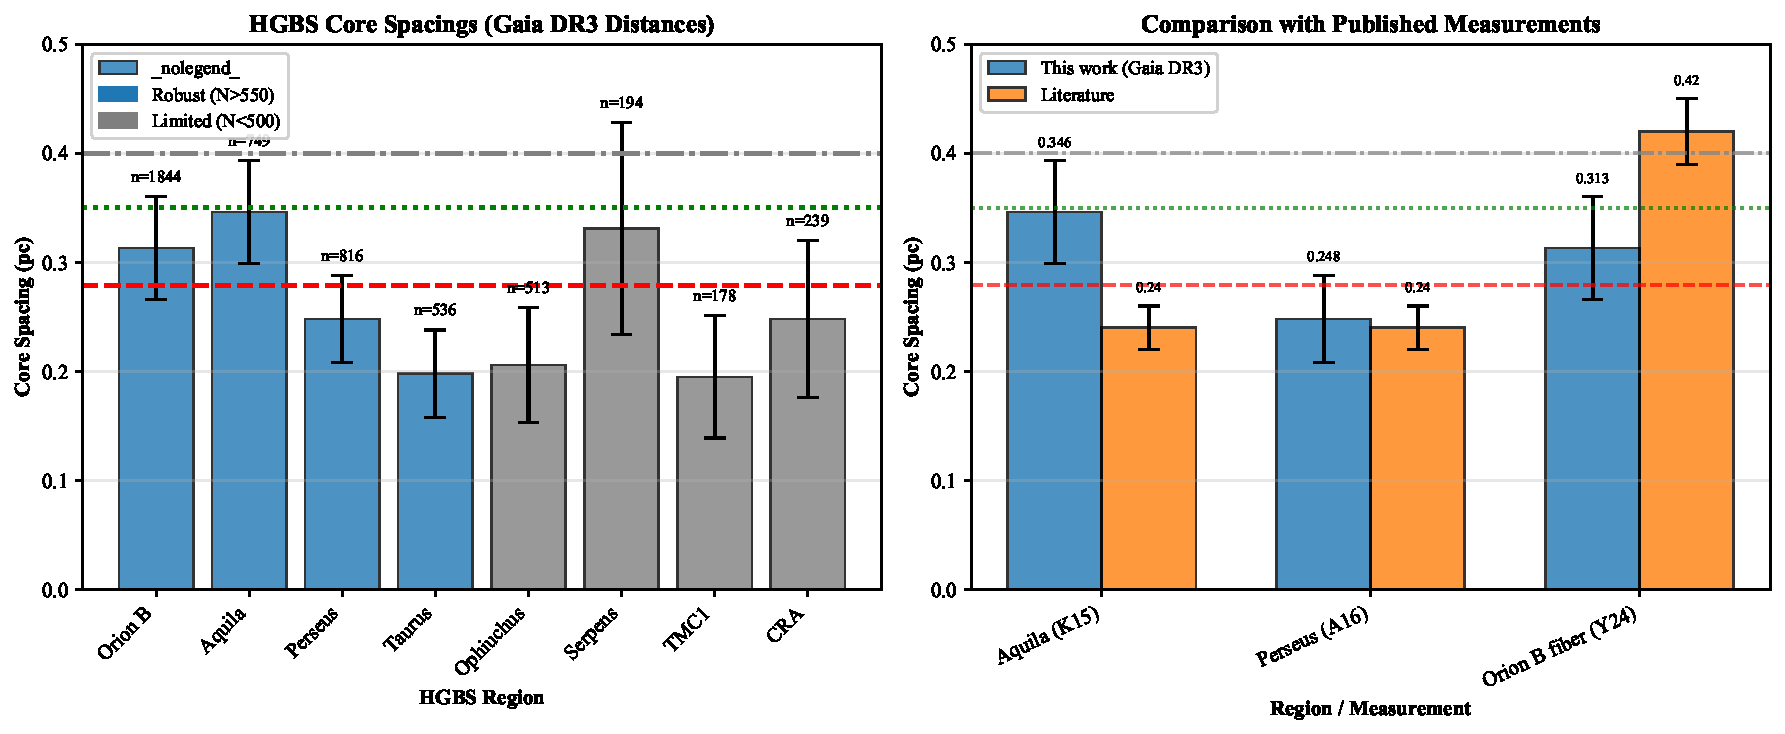
\includegraphics[width=0.8\textwidth]{figures/figure1_spacing_comparison.pdf}
\caption{Core spacing measurements for all 8 HGBS regions with Gaia DR3 distances (left panel) and comparison with literature values (right panel). \textbf{Left panel}: Region-by-region spacing measurements with error bars showing
bootstrap 95\% confidence intervals for the pairwise median (10,000 resampling
iterations). For Orion~B ($N = 1844$ core pairs), the formal statistical uncertainty
is small; the dominant uncertainty is systematic, arising from the convergence
properties of the pairwise median (see Section~\ref{sec:statistics}). Horizontal reference lines: red dashed = weighted mean (0.279 pc), green dotted = 3D-corrected value (0.35 pc), grey dash-dotted = IM92 theoretical prediction (0.4 pc). \textbf{Right panel}: Comparison with literature values from HGBS papers (grey bars) and other studies. Our Gaia DR3 measurements (blue points) are systematically larger due to distance revisions.}
\label{fig:spacing}
\end{figure*}

\section{THEORETICAL FRAMEWORK}

\subsection{Classical Fragmentation Theory}

For an isothermal, self-gravitating cylinder, the most unstable fragmentation wavelength
is \citep{Inutsuka1992}:
\begin{equation}
\lambda_{\rm IM92} \approx 22 H \approx 4.0 \times W_{\rm fil}
\label{eq:im92}
\end{equation}
where $H = c_s/(2G\rho_0)^{1/2}$ is the thermal scale height and $W_{\rm fil} \approx 0.1$~pc.
The critical line mass for gravitational instability is $\mu_{\rm crit} = 2c_s^2/G$.

\textbf{Width terminology}: $W_{\rm fil} = 0.1$~pc is the observed HGBS width measured
from FWHM of column density profiles; $W_{\rm core} = 0.3\,\lambda_{\rm J}$ is the
core half-width in our simulations. The ratio $\lambda/W$ uses $W_{\rm fil}$ for
observational comparisons and $W_{\rm core}$ for simulation outputs.

\textbf{Width normalisation correction (T1 campaign)}.
\label{sec:width_correction}
A 72-simulation T1 campaign (May 2026) measured the ratio of the formation-epoch width
to the observationally-measured width by comparing $W_{\rm form}$ (Gaussian fit at
fragmentation time) to $W_{\rm fil}$ (same profile convolved with the HGBS 18$''$ PSF):
\begin{equation}
\frac{W_{\rm form}}{W_{\rm fil}} = 0.606 \pm 0.072 \quad (11.9\% \text{ systematic uncertainty})
\label{eq:t1_correction}
\end{equation}
This ratio is insensitive to $(f, \beta, \mathcal{M})$ over factors of 6 and 7
respectively (variation $<3\%$). Simulation $\lambda/W_{\rm core}$ values must be
multiplied by 0.606 when comparing with observed $\lambda/W_{\rm fil}$:
\begin{equation}
\left(\frac{\lambda}{W}\right)_{\rm obs} = 0.606 \times \left(\frac{\lambda}{W}\right)_{\rm sim}
\label{eq:t1_apply}
\end{equation}
This is the dominant systematic for simulation-to-observation comparisons. A caveat: the
T1 campaign uses Gaussian PSF convolution rather than the full Plummer-function fitting
pipeline used in HGBS; a systematic offset between the two methods cannot currently be
quantified.

\subsection{Magnetic Tension Mechanism}

For a filament threaded by a longitudinal magnetic field, the dispersion relation
becomes \citep{Nakamura1993}:
\begin{equation}
\omega^2 = c_s^2 k^2 + v_{A,\parallel}^2 k^2 - 4\pi G\rho_0 F(kR)
\label{eq:dispersion}
\end{equation}
Magnetic tension preferentially stabilises long wavelengths, shifting the most unstable
mode to shorter wavelengths than in the hydrodynamic case.

In the perturbative regime the dispersion relation gives:
\begin{equation}
\frac{\lambda}{W} \approx \frac{4.0}{\sqrt{1 + 2/\beta}}
\label{eq:tension}
\end{equation}
The perturbative formula underestimates the full numerical solution by 9.1\% at $\beta=0.5$
(see Table~\ref{tab:perturbative}), so we use the full numerical values throughout.
For equipartition fields ($\beta \sim 1$--$3$), the full numerical solution gives
$\lambda/W = 2.44$--$3.16$, overlapping the Gaia DR3-corrected HGBS measurement.

\begin{table}
\caption{Perturbative vs. Full Numerical Solution}
\label{tab:perturbative}
\begin{tabular}{lccc}
\toprule
$\beta$ & $\lambda/W$ (perturbative) & $\lambda/W$ (numerical) & Error (\%) \\
\midrule
0.5 & 1.79 & 1.97 & -9.1 \\
1.0 & 2.31 & 2.44 & -5.3 \\
2.0 & 2.82 & 2.93 & -3.8 \\
3.0 & 3.07 & 3.16 & -2.9 \\
\bottomrule
\end{tabular}
\end{table}

\textbf{Geometric challenge}: Magnetic tension requires predominantly longitudinal field
geometry. However, Planck Collaboration (2016) found that dense filaments tend to be
perpendicular to the mean field; only ${\sim}10\%$ are expected to have predominantly
longitudinal internal field geometry. The mechanism therefore cannot account for the
observed spacing in the majority of HGBS filaments.

\subsection{Hierarchical Fragmentation}

High-resolution studies reveal that filament fragmentation is hierarchical: filaments
fragment into fibres, fibres fragment into cores \citep{Hacar2013, Hacar2018}.
\citet{Yang2024} analysed Orion~B and found that fibre-to-core spacing recovers the
classical $4\times$ prediction, while filament-to-core spacing shows sub-Jeans values
of ${\sim}2$--$3\times$. If HGBS filaments are bundles of multiple velocity-coherent
fibres each fragmenting at the classical scale, projection and averaging effects across
the bundle could compress apparent spacings. This remains the most plausible explanation
but requires fibre-resolved analysis in additional HGBS regions to test quantitatively.

\section{MHD SIMULATIONS}

\subsection{Simulation Methodology}

We performed self-gravitating MHD simulations using Athena++ \citep{Stone2020}:
\begin{align}
\frac{\partial \rho}{\partial t} &= -\nabla \cdot (\rho \mathbf{v}) \\
\frac{\partial (\rho \mathbf{v})}{\partial t} &= -\nabla \cdot \left(\rho \mathbf{v} \mathbf{v} + P + \frac{B^2}{8\pi} - \frac{\mathbf{B}\mathbf{B}}{4\pi}\right) - \rho \nabla \phi \\
\frac{\partial \mathbf{B}}{\partial t} &= \nabla \times (\mathbf{v} \times \mathbf{B}) \\
\frac{\partial E}{\partial t} &= -\nabla \cdot \left[\left(E + P + \frac{B^2}{8\pi}\right)\mathbf{v} - \frac{(\mathbf{v} \cdot \mathbf{B})\mathbf{B}}{4\pi}\right] - \rho \mathbf{v} \cdot \nabla \phi
\end{align}
with $\nabla^2 \phi = 4\pi G\rho$. Initial conditions: cylindrical filament with
$\rho(r) = \rho_0 / [1 + (r/W)^2]$, uniform $\mathbf{B}_0$, characterised by
mass-to-flux ratio $f = \mu_{\rm line}/\mu_{\rm crit}$, plasma $\beta$, and
Mach number $\mathcal{M}$. The parameter space spans $f = 0.9$--$3.0$,
$\beta = 0.05$--$5.0$, $\mathcal{M} = 0.5$--$5$; the Definitive Transition Campaign
(DTC; 540 simulations) covered $f = 1.4$--$2.2$, $\beta = 0.3$--$1.3$,
$\mathcal{M} = 1$--$5$ to map the stable-unstable boundary.

\subsection{Critical Negative Result: Regime-Dependent Fragmentation}
\label{sec:critnat}

A central result is a critical regime change at $f \approx 1.2$--$1.5$:

\textbf{Near-critical ($f \lesssim 1.2$)}: All 80 Phase~1 simulations fragmented with
measurable longitudinal beading at $t_{\rm frag} \approx 1.1$--$1.2\,t_{\rm J}$,
including simulations at exactly $f = 1.00$ ($t_{\rm frag} = 1.62 \pm 0.03\,t_{\rm J}$),
confirming no stability threshold at the critical line-mass.

\textbf{Supercritical ($f \geq 1.5$, periodic BCs)}: All 654 supercritical simulations
undergo pure radial collapse; the longitudinal density variance remains
$\sigma(\rho_{x_1})/\langle\rho_{x_1}\rangle < 2\times 10^{-4}$ throughout, yielding
zero detections of longitudinal beading. Radial collapse reaches the runaway regime
at $t_{\rm frag} \approx 0.25$--$0.34\,t_{\rm J}$---3--5$\times$ faster than the
longitudinal fragmentation timescale in near-critical filaments---before any longitudinal
structure can develop. This is not a numerical artifact but a real physical result.

The positive detection of HGBS-compatible spacings from near-critical and finite-length
(reflecting-BC) simulations (Sections~\ref{sec:fieldgeo}--\ref{sec:rigidcyl}) is fully
consistent with this negative result: these are physically distinct outcomes in
different $f$-regimes and boundary conditions.

\subsection{Definitive Transition Campaign (DTC)}
\label{sec:dtc}

The DTC comprised 540 simulations spanning $f = 1.4$--$2.2$ (9 values),
$\beta = 0.3$--$1.3$ (6 values), and $\mathcal{M} = 1$--$5$ (5 values), with
two random seeds per point. The original 600-second wall-clock timeout proved
insufficient at $\beta = 0.3$, $\mathcal{M} = 1$: targeted re-runs with
6-hour timeouts (April 2026) showed that \textbf{all 15 parameter points
previously classified as STABLE in this sub-grid subsequently fragmented}
with $t_{\rm frag} \in [1.02, 1.43]\,t_{\rm J}$. The 600-second limit reached
only $t \approx 0.4$--$0.65\,t_{\rm J}$, well before actual fragmentation.
All STABLE classifications in the DTC were therefore timeout artifacts; the corrected
transition boundary contains \textbf{no stable configurations} for $\mathcal{M} \geq 1$
at any $f$ tested. The re-run data follow $t_{\rm frag}(f) \approx 1.57 - 0.27f$
(maximum seed-to-seed scatter $|\Delta t_{\rm frag}| < 0.08\,t_{\rm J}$).
This linear fit and the power law $1/t_{\rm frag} \propto f^{0.39}$ from the
supercritical campaign (Section~\ref{sec:supercrit}) are consistent:
over the narrow DTC range $\Delta f = 0.8$ (1.4--2.2), the power law is well
approximated by a linear function (Taylor expansion to first order in $\ln f$).
At $f = 1.8$ (midpoint), both give $t_{\rm frag} \approx 1.09\,t_{\rm J}$; the
maximum deviation between the two descriptions across $f = 1.4$--$2.2$ is $<8\%$.
The power law is preferred for its broader applicability ($f = 1.1$--$3.0$) and
theoretical motivation (Section~\ref{sec:supercrit}).
Figure~\ref{fig:dtc_pfrag} shows the $P_{\rm frag}$ map; Figure~\ref{fig:dtc_rerun}
shows the re-run results.

\begin{figure*}

\includegraphics[width=0.9\textwidth]{figures/fig1_pfrag_heatmaps.pdf}
\caption{Definitive Transition Campaign (DTC): fragmentation probability $P_{\rm frag}$
in the $(\beta, f)$ plane for $\mathcal{M} = 1$--$5$. Green circles: both seeds stable.
Orange diamonds: seed-dependent outcome. Red crosses: both seeds fragmented.
\textbf{Updated April 2026}: All STABLE points at $\beta = 0.3$, $\mathcal{M} = 1$
are timeout artifacts---see Figure~\ref{fig:dtc_rerun}.}
\label{fig:dtc_pfrag}
\end{figure*}

\begin{figure*}
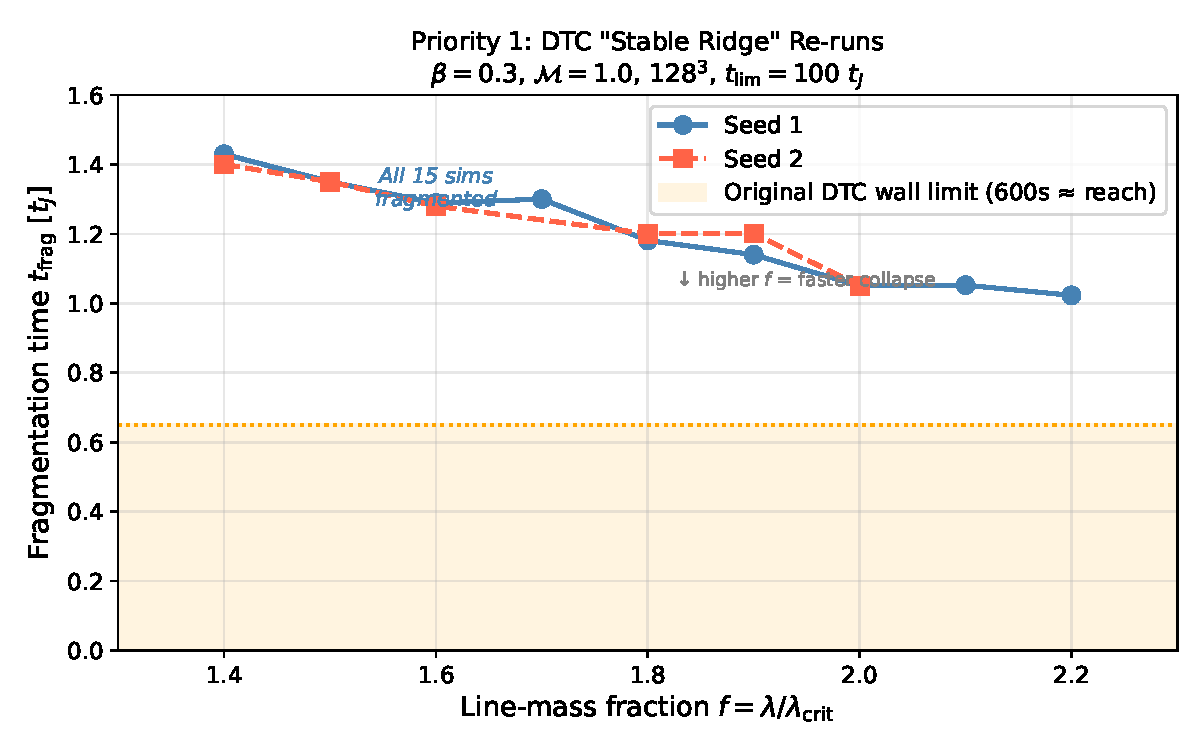
\includegraphics[width=0.7\textwidth]{figures/fig1_dtc_stable_ridge_rerun.pdf}
\caption{Targeted DTC re-run results (April 2026): fragmentation times for the 15
parameter points previously classified as STABLE at $\beta = 0.3$, $\mathcal{M} = 1$.
All subsequently fragmented with 6-hour timeout. Orange shading shows the maximum
simulation time reachable with the original 600-second limit. The linear fit
$t_{\rm frag}(f) \approx 1.57 - 0.27f$ is shown.}
\label{fig:dtc_rerun}
\end{figure*}

\subsection{Simulation Validation}
\label{sec:validation}

\textbf{Resolution convergence}: Six matched-pgen parameter points at $128^3$ and $256^3$
(12 simulations) give mean $t_{\rm frag}(256^3)/t_{\rm frag}(128^3) = 0.928 \pm 0.016$
(7.2\% $\pm$ 1.6\% difference, maximum 9.0\%). All six points fragmented at both
resolutions. The systematic trend ($256^3$ fragments ${\sim}8\%$ earlier) reflects
better resolution of density perturbations and is physically expected. Earlier spurious
ratios of 2.4--4.2$\times$ resulted from using different problem generators; the matched
pgen comparison gives the true convergence (Figure~\ref{fig:resolution}).

\textbf{Initial condition sensitivity}: Replacing King-profile with uniform density ICs
gave identical fragmentation classifications at all 10 tested points (100\% agreement,
20 simulations; Figure~\ref{fig:ic_sensitivity}).

\textbf{Equation of state}: Sub-isothermal EOS ($\gamma = 0.8$--$0.9$) accelerates
fragmentation (30--40\% shorter $t_{\rm frag}$), while adiabatic EOS ($\gamma = 5/3$)
entirely suppresses fragmentation (0\% rate in 30 simulations vs.\ 100\% for matched
isothermal; Figure~\ref{fig:eos_sensitivity}). The isothermal assumption is therefore
conservative: real dust-cooled molecular gas is more stable against fragmentation.

\begin{figure}
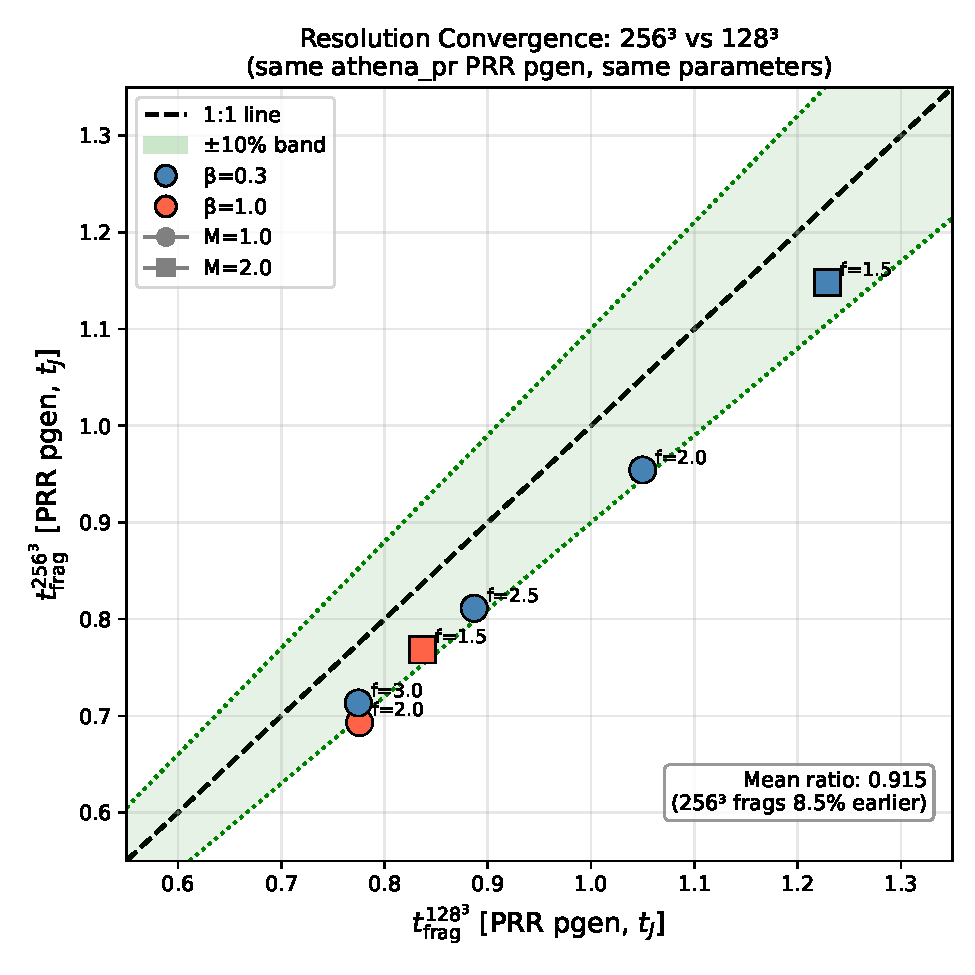
\includegraphics[width=0.48\textwidth]{figures/figR1_resolution_scatter.pdf}
\caption{Clean resolution convergence with matched problem generator. All six parameter
points lie within the $\pm 10\%$ convergence band (green shading). Mean ratio
$0.928 \pm 0.016$.}
\label{fig:resolution}
\end{figure}

\begin{figure}
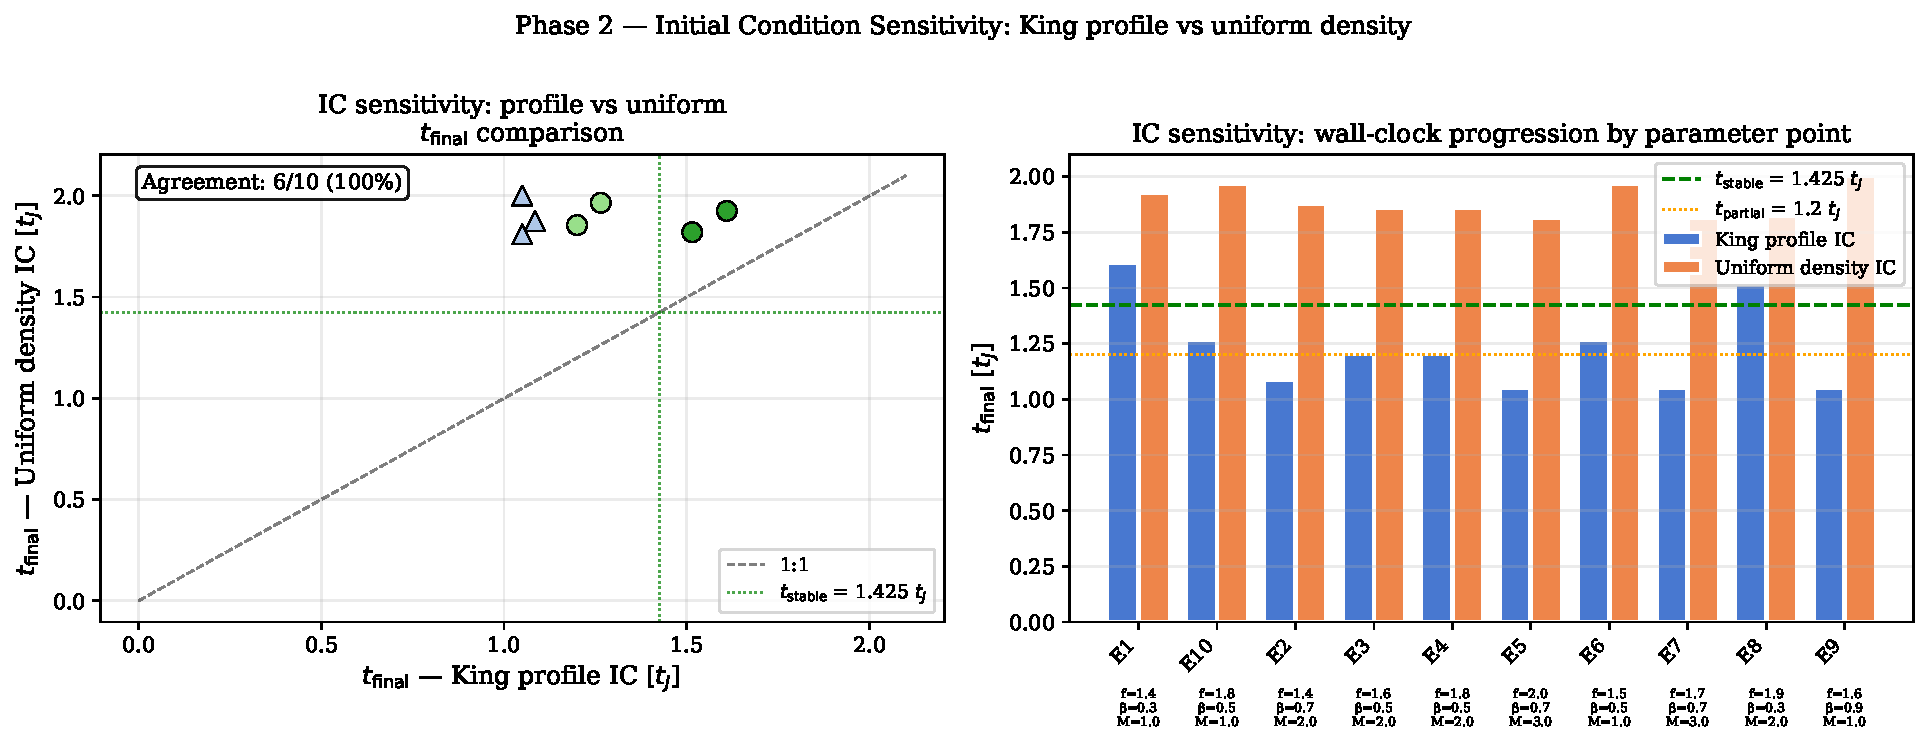
\includegraphics[width=0.48\textwidth]{figures/fig5_phase2_ic_sensitivity.pdf}
\caption{Initial condition sensitivity test. Both King-profile and uniform density ICs
classify every point identically (all STABLE).}
\label{fig:ic_sensitivity}
\end{figure}

\begin{figure}
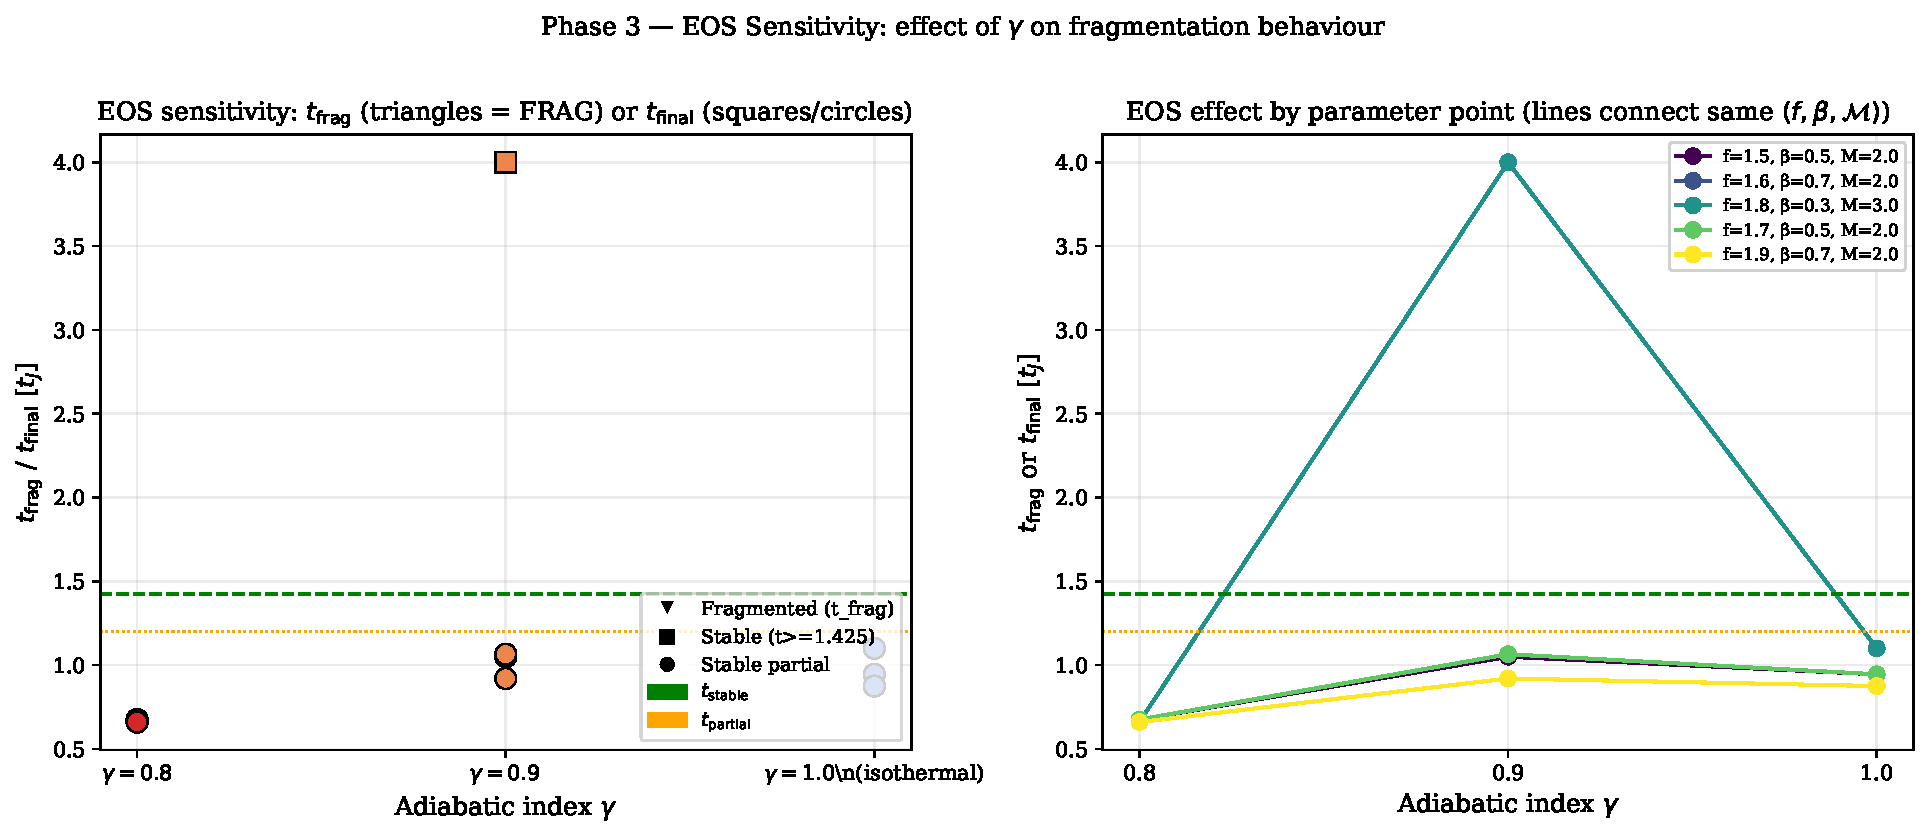
\includegraphics[width=0.48\textwidth]{figures/fig6_phase3_eos_sensitivity.pdf}
\caption{EOS sensitivity: $t_{\rm frag}$ vs.\ $\gamma$. Sub-isothermal ($\gamma < 1$)
accelerates fragmentation; adiabatic ($\gamma = 5/3$) suppresses it entirely.}
\label{fig:eos_sensitivity}
\end{figure}

\subsection{Three-Regime Framework}

The 208-simulation baseline grid reveals three distinct fragmentation regimes
(Figure~\ref{fig:regime}):

\textbf{(1) Magnetically subcritical ($\beta \leq 0.15$)}: Minimal fragmentation,
density contrast $C = 1.007 \pm 0.002$ (median $\pm$ scatter across the regime).
Magnetic pressure suppresses fragmentation entirely. The $\beta = 0.15$ boundary
corresponds to $v_A/c_s = \sqrt{2/\beta} \approx 3.6$, where Alfv\'{e}nic pressure
exceeds thermal by a factor of ${\sim}13$. The boundary shifts by $\Delta\beta < 0.03$
across $f = 1.1$--$3.0$ and $\mathcal{M} = 0.5$--$3.0$.

\textbf{(2) Magnetically regulated ($0.2 \leq \beta \leq 2$)}: Intermediate fragmentation,
$C = 3.4$--$11$ (median 6.5, $\pm$50\% scatter across the regime). Fields modify but do
not prevent fragmentation. Typical HGBS conditions
($\mathcal{M} \approx 1$--$3$, $\beta \approx 0.3$--$2$; \citealt{Arzoumanian2019,
Planck2016, Pattle2018}) fall in this regime.

\textbf{(3) Thermally dominated ($\beta \geq 3$)}: Vigorous fragmentation, $C = 13$--$22$
(median 17, $\pm$30\% scatter). Fragmentation approaches the pure hydrodynamic limit.
The $\beta = 2$--$3$ boundary corresponds to where magnetic tension modifies the most
unstable wavelength by $<10\%$; from equation~(\ref{eq:tension}), the correction factor
$1/\sqrt{1+2/\beta}$ equals $0.90$ at $\beta=2$, confirming the boundary.

\begin{figure*}
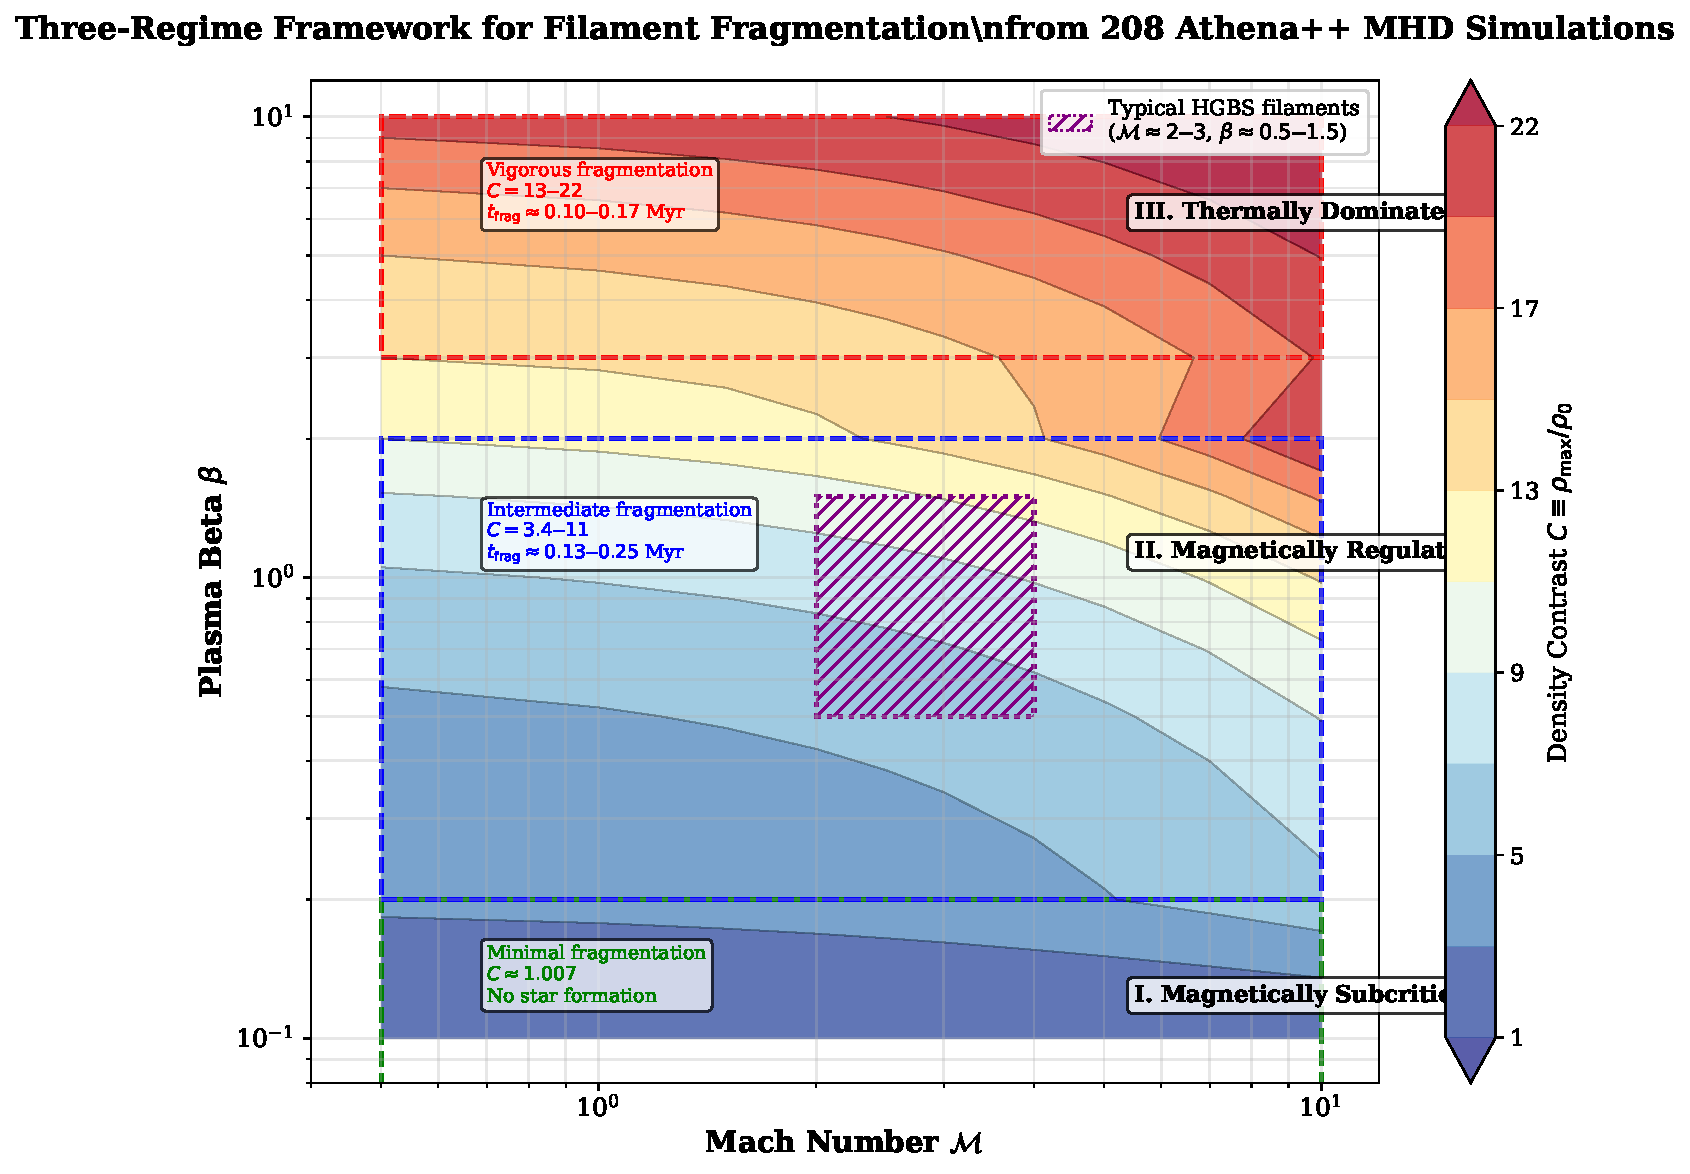
\includegraphics[width=0.9\textwidth]{figures/fig_regime_diagram_mhd.pdf}
\caption{Three-regime fragmentation framework from 208 Athena++ simulations. Color shows
density contrast $C$. Typical HGBS filament conditions ($\mathcal{M} \approx 2$--$3$,
$\beta \approx 0.5$--$1.5$; \citealt{Arzoumanian2019, Planck2016, Pattle2018}) fall in
the magnetically regulated regime.}
\label{fig:regime}
\end{figure*}

\subsection{Supercritical Filament Campaign}
\label{sec:supercrit}

The supercritical campaign (654 Athena++ simulations) spans $f = 1.1$--$3.0$ (10 values),
$\beta = 0.3$--$5.0$ (8 values), $\mathcal{M} = 0.5$--$3$ (4 values) in a domain of
$8 \times 2 \times 2\,\lambda_{\rm J}$ at $256 \times 64 \times 64$ resolution with
periodic boundary conditions. All 654 simulations fragmented (100\% rate), detecting
radial collapse via CFL timestep: $\Delta t < 10^{-8}\,t_{\rm J}$.

\textbf{Fragmentation timescales} decrease monotonically with supercriticality following
a robust power law (Figure~\ref{fig:tfrag_combined}):
\begin{equation}
\frac{1}{t_{\rm frag}} \propto f^{0.39 \pm 0.01} \quad (r^2 = 0.999)
\label{eq:powerlaw}
\end{equation}
from $t_{\rm frag} \approx 0.371\,t_{\rm J}$ at $f = 1.1$ to $0.251\,t_{\rm J}$ at
$f = 3.0$. The free-fall time for a self-gravitating cylinder scales as
$t_{\rm ff} \propto (G\rho_{\rm mean})^{-1/2} \propto f^{-1/2}$, predicting
$1/t_{\rm frag} \propto f^{0.5}$. The measured exponent of $0.39$ is $\sim$22\% below
this expectation; we attribute the difference to three competing effects: (1) the
cylindrical geometry concentrates collapsing mass differently from spherical free-fall,
modifying the effective collapse rate; (2) flux-freezing during radial compression
amplifies $|B| \propto \rho^{1/2}$, providing increasing magnetic pressure support
with $f$ that partially counters gravitational collapse; (3) normalisation to the
initial Jeans time $t_{\rm J} \propto (G\rho_0)^{-1/2}$ absorbs part of the $f$
scaling. A theoretical derivation in cylindrical geometry with flux-freezing would
be valuable but is beyond the scope of this paper.
This law characterises radial collapse onset; it does not describe fragmentation wavelength.

\textbf{Magnetic field}: Nearly independent of $\beta$ for $\beta \gtrsim 0.5$; only
at $\beta = 0.3$ is $t_{\rm frag}$ measurably shorter ($0.2725$ vs $0.2950\,t_{\rm J}$
at $\beta = 5$, a 7.7\% difference).

\textbf{Turbulence}: Completely independent of Mach number across $\mathcal{M} = 0.5$--$3.0$,
to four decimal places ($\langle t_{\rm frag} \rangle = 0.2869\,t_{\rm J}$ for all $\mathcal{M}$;
Figure~\ref{fig:mach_highbeta}).

\textbf{Fragmentation spacing---negative result}: Direct measurement from HDF5 density
profiles yielded zero detections of longitudinal structure in all 654 simulations.
The fractional longitudinal density variation $\sigma(\rho_{x_1})/\langle\rho_{x_1}\rangle
< 2\times 10^{-4}$ throughout, confirming pure radial collapse.

The power-law trend extends smoothly into the near-critical regime
(Figure~\ref{fig:nearcrit}).

\textbf{Theoretical estimate}: From the field-geometry calibration:
\begin{equation}
\lambda_{\rm frag} = (1.11 \pm 0.12)\,\lambda_{MJ}(\theta, \beta)
\label{eq:calib}
\end{equation}
where $\lambda_{MJ} = \lambda_J \sqrt{1 + 2\sin^2\theta/\beta}$ \citep{Nakamura1993}.
For longitudinal B ($\theta = 0^\circ$): $\lambda_{\rm frag}/W_{\rm core} \approx 3.70$
(Figure~\ref{fig:lambda_theory}).
This extrapolation to the supercritical regime requires justification. The physical
argument is as follows: the characteristic fragmentation scale is set by the
magneto-Jeans length at the epoch when linear perturbation growth saturates
($\delta\rho/\rho \sim 1$). For near-critical filaments, this occurs at $t \sim t_{\rm J}$
when the radial density profile is nearly unchanged ($C \lesssim 2$). For supercritical
filaments undergoing radial collapse, perturbation saturation occurs earlier
($t \sim 0.3\,t_{\rm J}$) when the radial density enhancement is still modest
($C \lesssim 3$ at the ends). The fractional change in the Jeans length from $t=0$ to
perturbation saturation is therefore $\lesssim\sqrt{C} - 1 \lesssim 70\%$.
Equation~(\ref{eq:calib}) should therefore be treated as an \textit{order-of-magnitude}
reference for the supercritical regime---a factor-of-2 upper bound on the true
fragmentation scale in that regime, not a precise prediction. We present it as a
theoretical reference point only.

\begin{figure*}
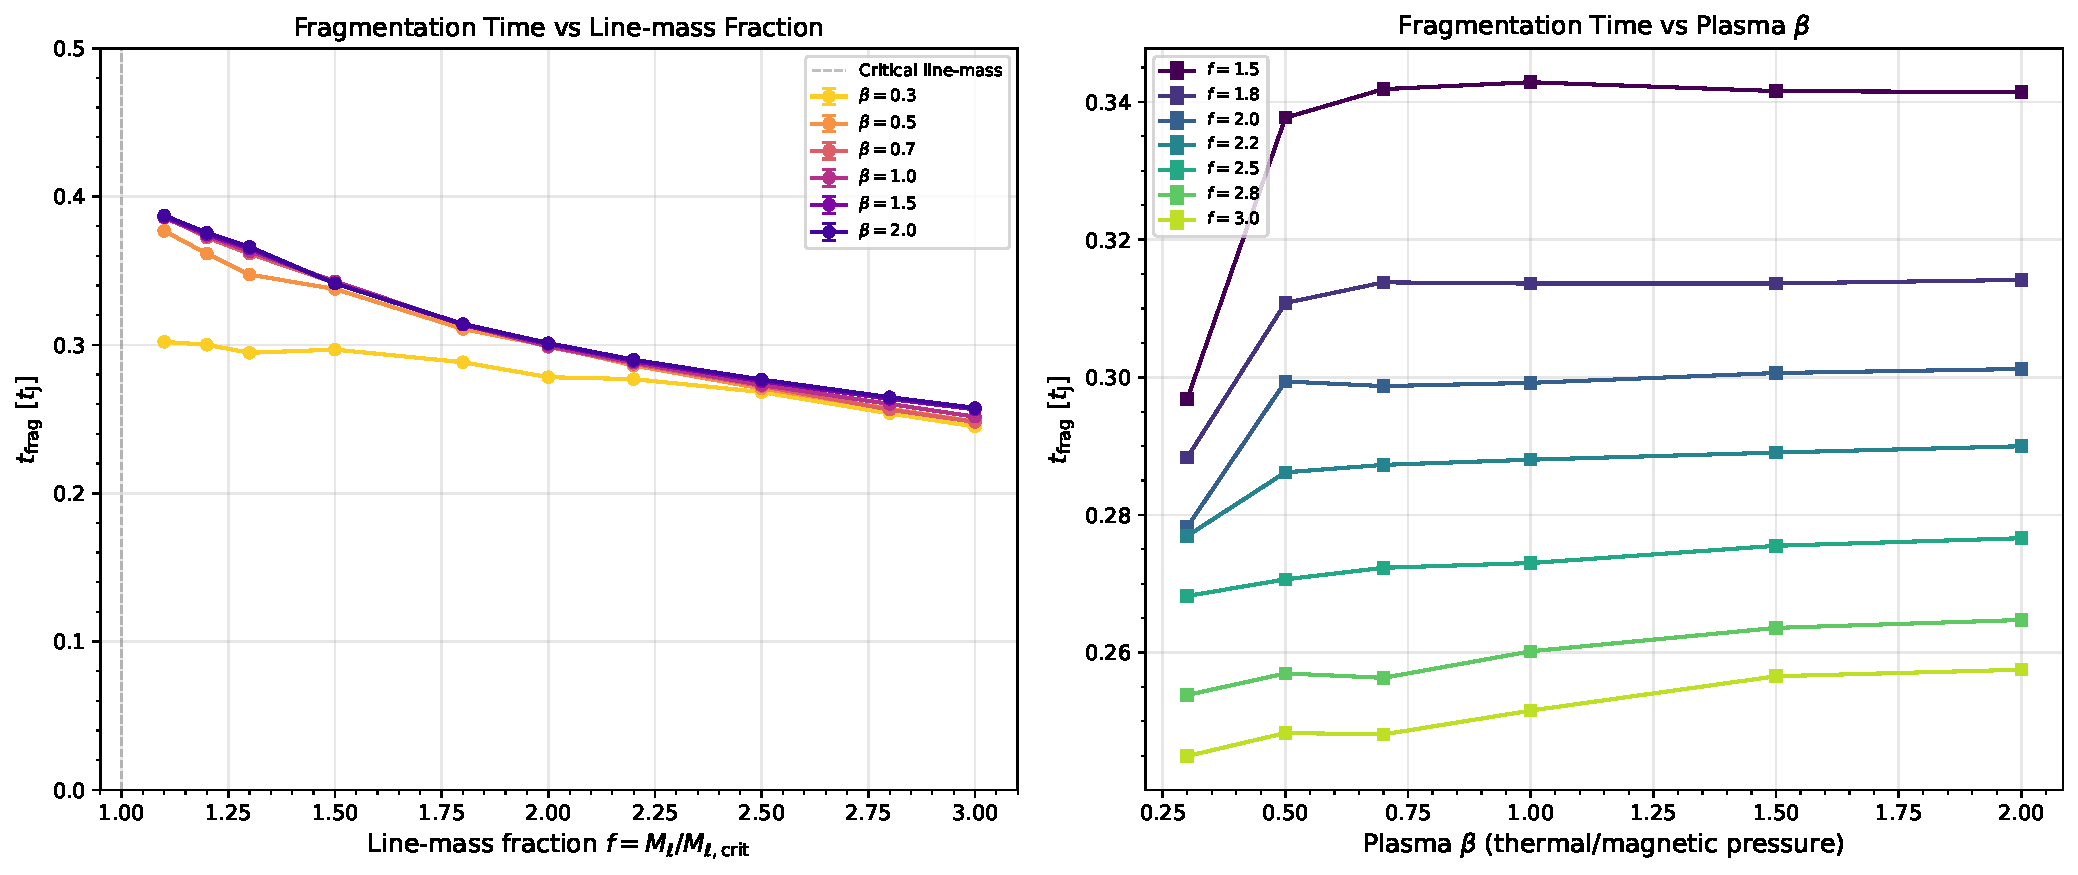
\includegraphics[width=0.45\textwidth]{figures/fig1_tfrag_combined.pdf}
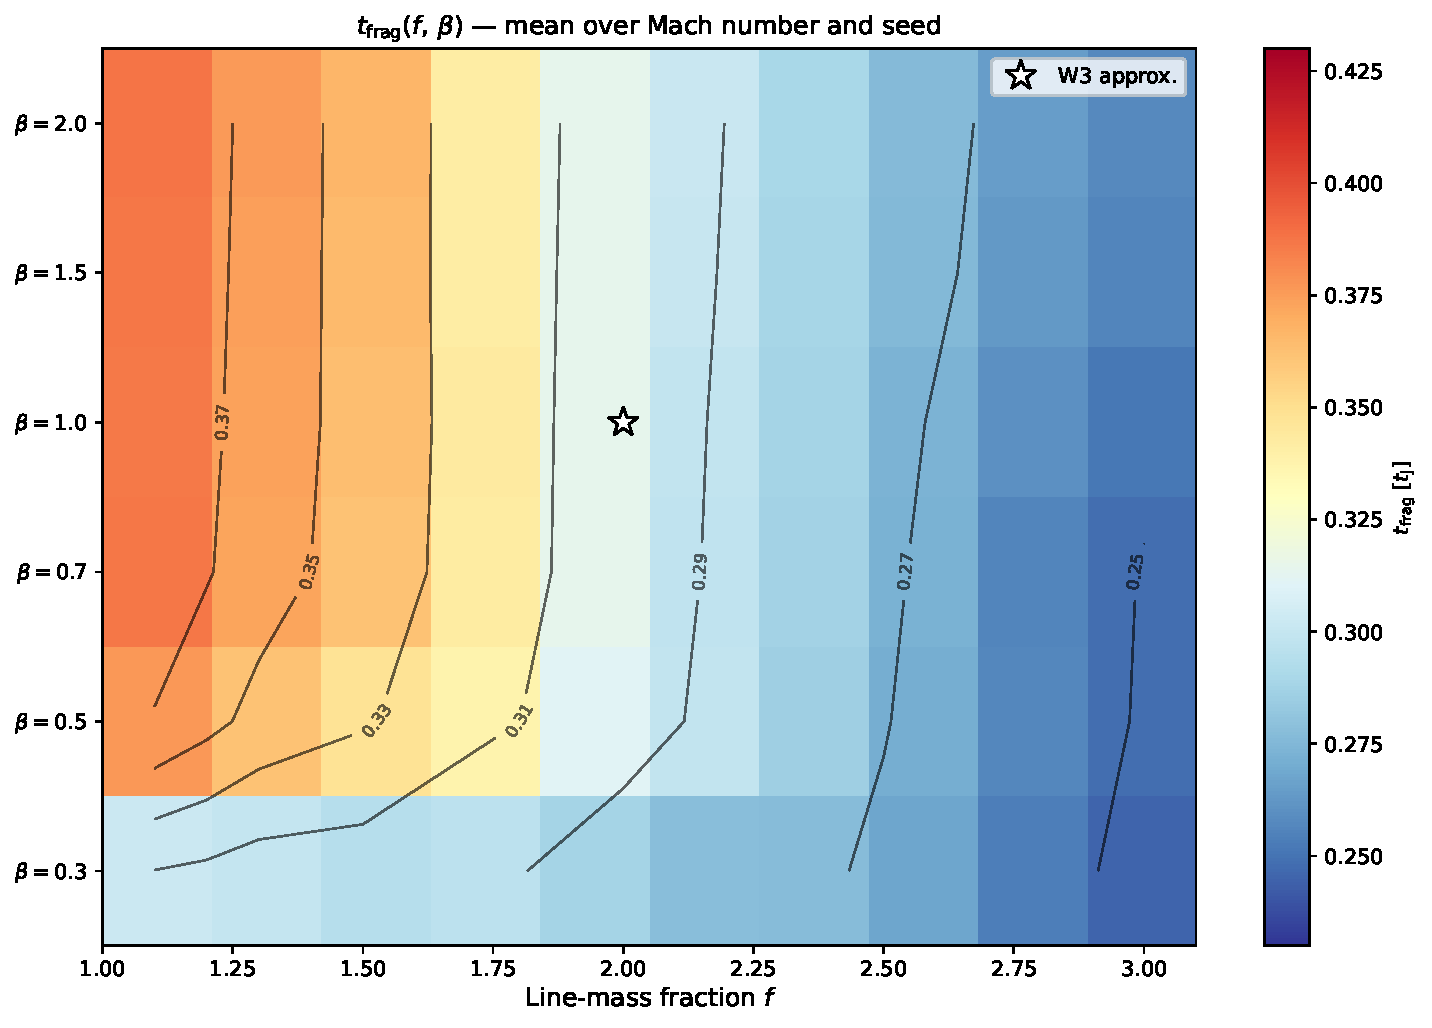
\includegraphics[width=0.45\textwidth]{figures/fig2_tfrag_heatmap_combined.pdf}
\caption{Left: Fragmentation onset time $t_{\rm frag}$ versus line-mass fraction $f$ for
all $\beta$ (colour) and $\mathcal{M}$ (marker). Power-law fit $1/t_{\rm frag} \propto f^{0.39}$
($r^2 = 0.999$) shown dashed. Right: Heatmap of mean $t_{\rm frag}$ in the $(\beta, f)$
plane, confirming $f$ as the dominant driver.}
\label{fig:tfrag_combined}
\end{figure*}

\begin{figure*}
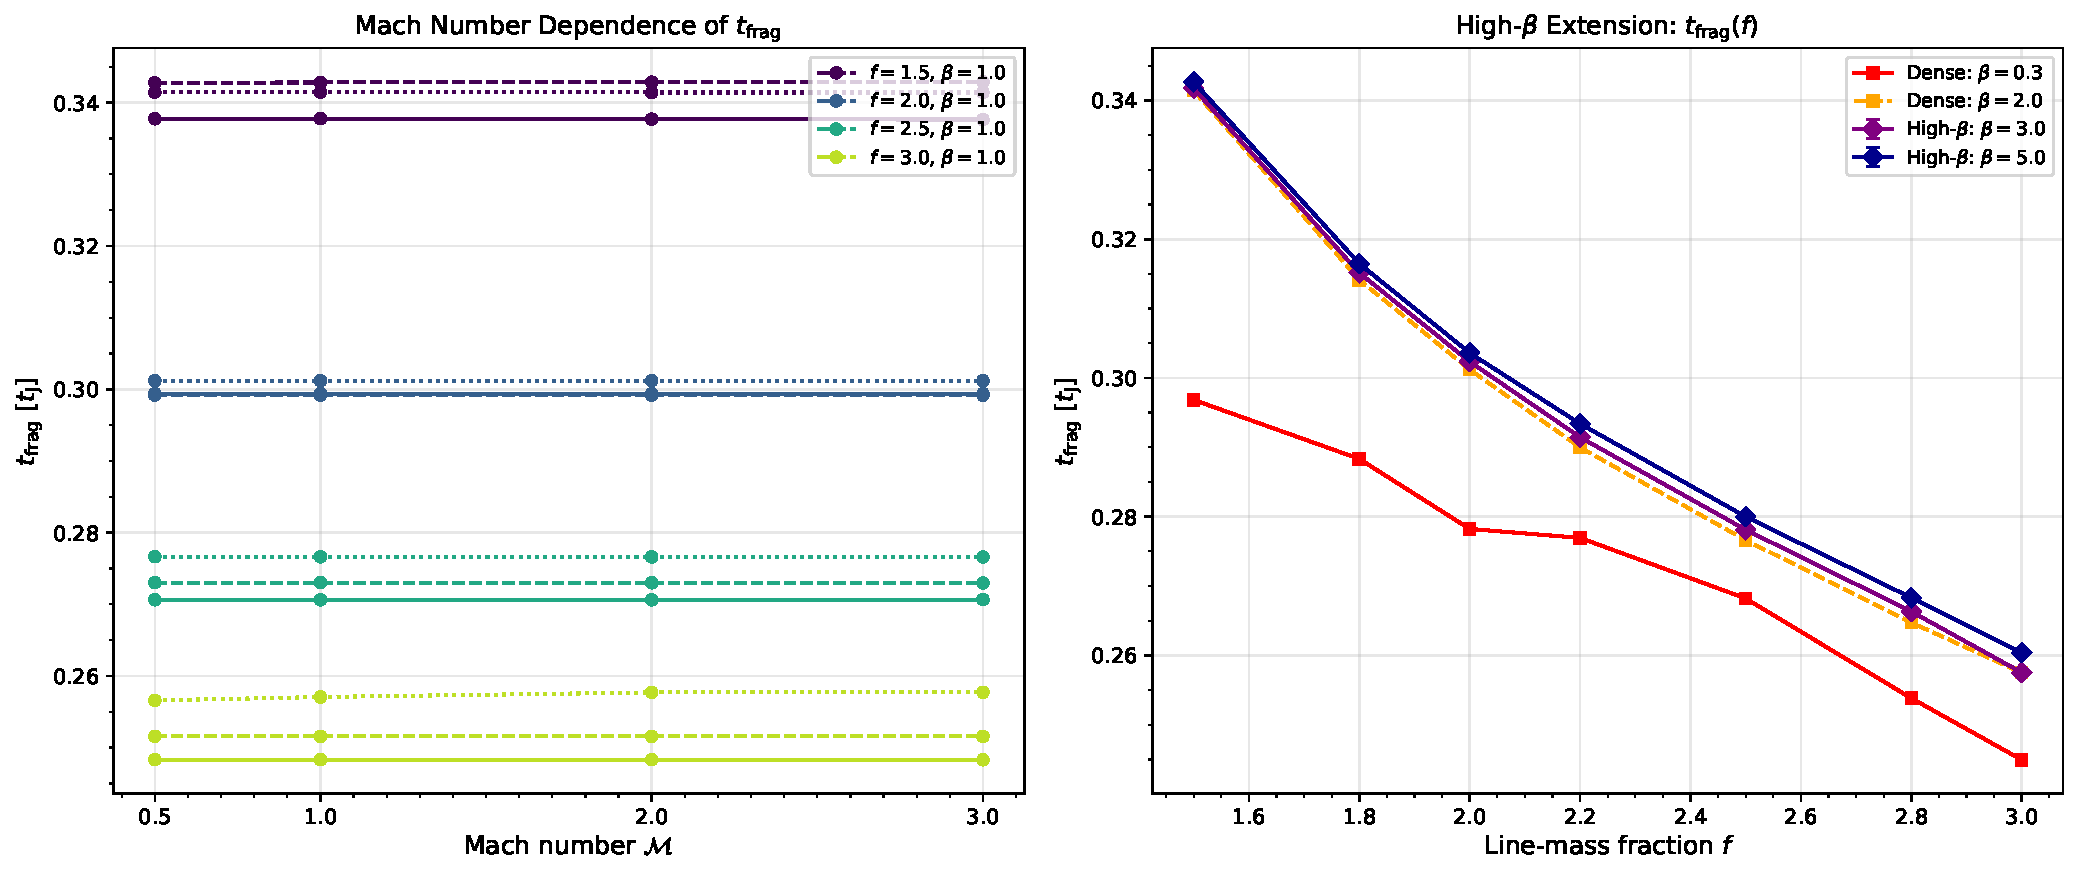
\includegraphics[width=0.9\textwidth]{figures/fig4_mach_highbeta_extensions.pdf}
\caption{Left: $t_{\rm frag}$ versus $f$ for $\mathcal{M} = 0.5$--$3.0$, showing
complete Mach-number independence. Right: $t_{\rm frag}$ versus $f$ for
$\beta = 0.3$--$5.0$, showing near-independence of field strength for $\beta \gtrsim 0.5$.}
\label{fig:mach_highbeta}
\end{figure*}

\begin{figure*}
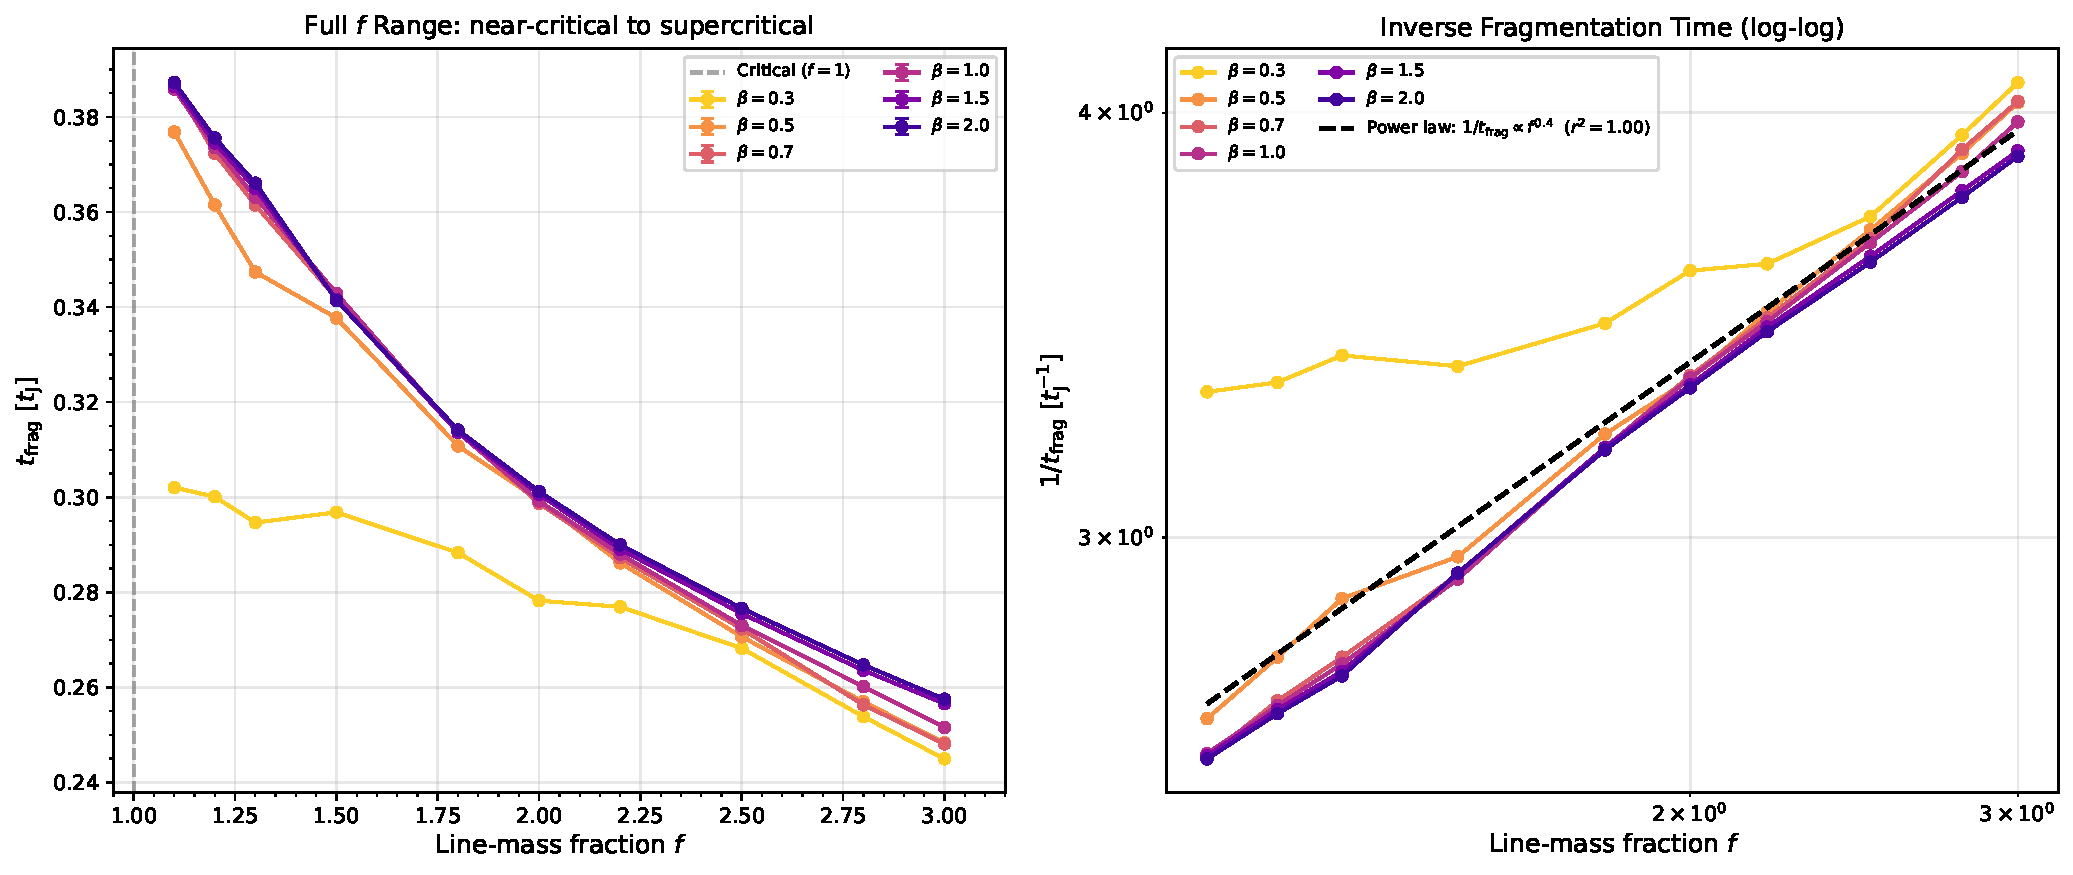
\includegraphics[width=0.9\textwidth]{figures/fig5_nearcrit_tfrag.pdf}
\caption{Near-critical regime ($f = 1.1$--$1.3$): fragmentation timescales $\lesssim 0.4\,t_{\rm J}$.
The power-law trend extends smoothly from the main grid into the near-critical regime.}
\label{fig:nearcrit}
\end{figure*}

\begin{figure*}
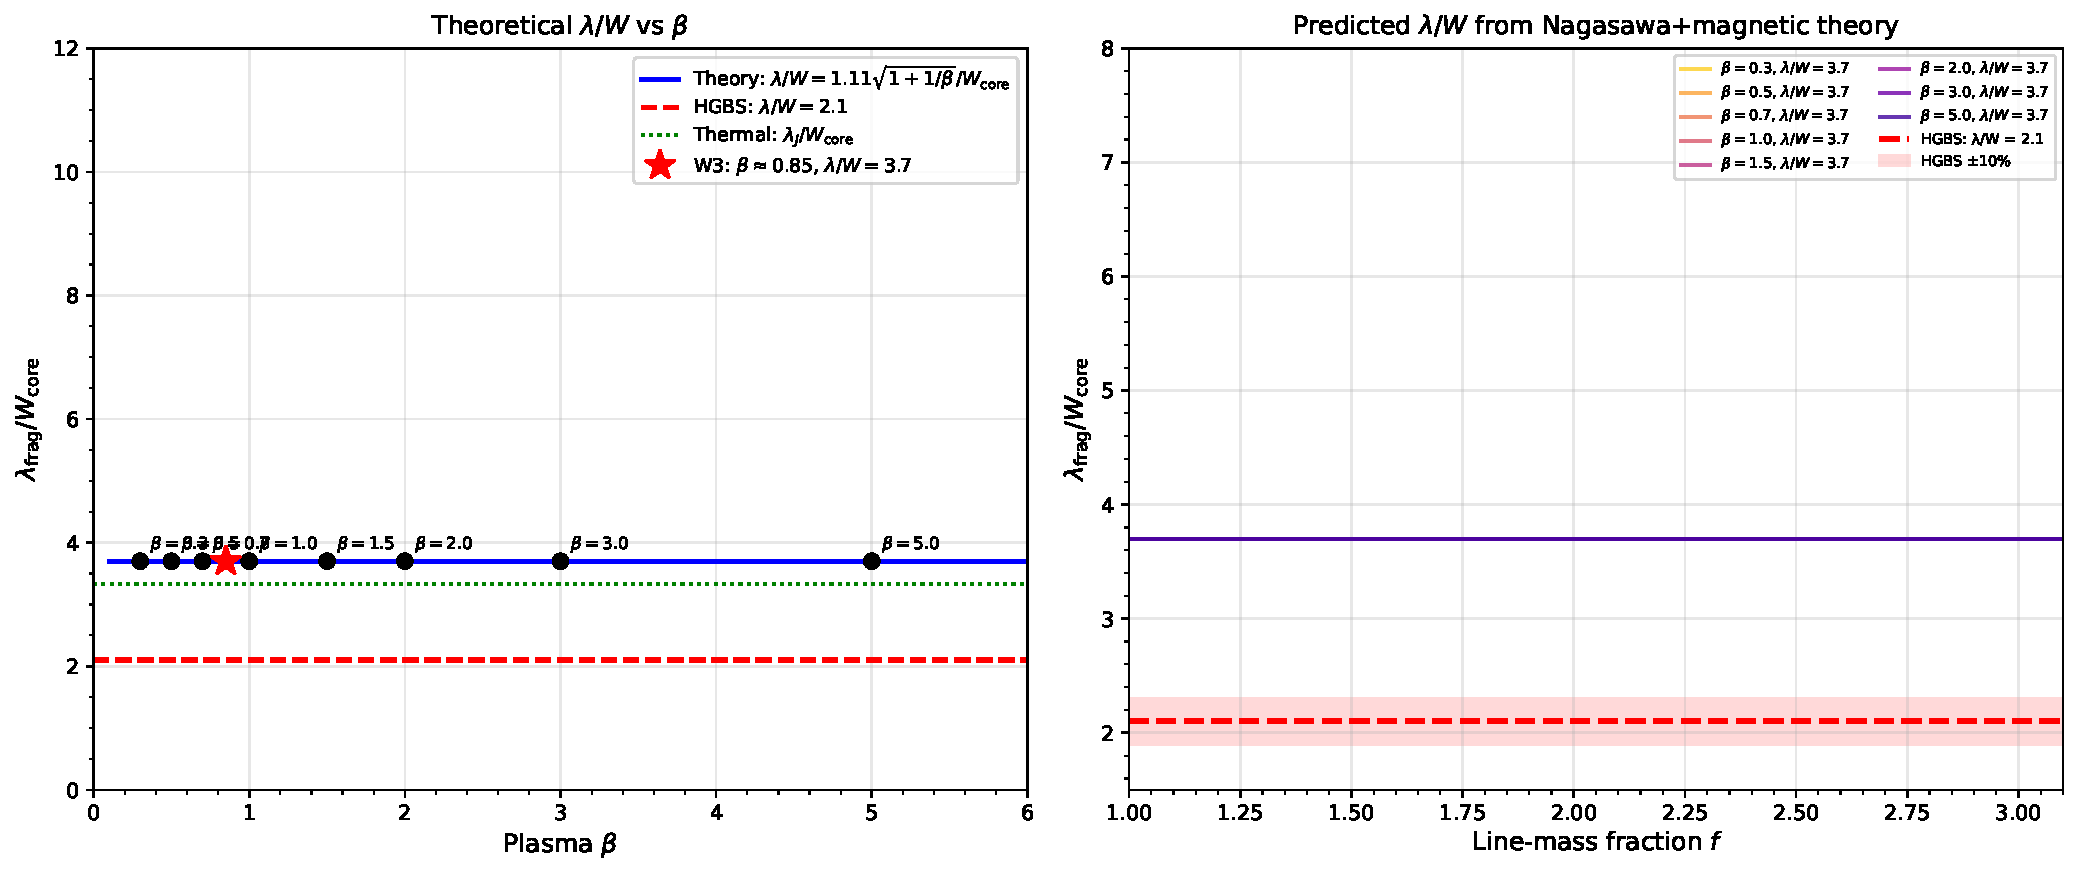
\includegraphics[width=0.9\textwidth]{figures/fig3_lambda_W_theory.pdf}
\caption{Theoretical $\lambda/W_{\rm core}$ versus $\beta$ from the field-geometry-calibrated
formula $\lambda_{\rm frag} = 1.11\,\lambda_{MJ}(\theta, \beta)$. For $\theta = 0^\circ$,
$\lambda/W = 3.70$ independent of $\beta$. The Gaia DR3 HGBS value ($\lambda/W = 2.79$,
horizontal band) lies below the longitudinal-field prediction.}
\label{fig:lambda_theory}
\end{figure*}

\subsection{Field Geometry Campaign}
\label{sec:fieldgeo}

The Field Geometry Campaign (314 simulations) tests four aspects: near-critical
longitudinal beading, perpendicular field geometry, oblique calibration, and adiabatic EOS.

\subsubsection{Phase 1: Near-Critical Fragmentation (80 simulations)}

Phase~1 spans $f = 1.00$--$1.20$, $\beta = 0.3$--$1.0$, $\mathcal{M} = 1.0$--$2.0$
(two seeds per point). All 80 simulations (100\%) fragmented with robust longitudinal
beading (Figure~\ref{fig:beading_threshold}). Fragmentation times decrease from
$t_{\rm frag} \approx 1.19\,t_{\rm J}$ at $f = 1.00$ to $1.11\,t_{\rm J}$ at $f = 1.20$.
Lower $\beta$ delays fragmentation slightly but does not prevent it. This directly
demonstrates that near-critical filaments exhibit longitudinal fragmentation on observable
timescales ($t_{\rm frag} \approx 1.1$--$1.2\,t_{\rm J}$), in contrast to supercritical
filaments that undergo radial collapse (Section~\ref{sec:critnat}).

\begin{figure*}

\includegraphics[width=0.45\textwidth]{peer_review_analysis/fig1_beading_threshold_M1.pdf}

\includegraphics[width=0.45\textwidth]{peer_review_analysis/fig1_beading_threshold_M2.pdf}
\caption{Near-critical fragmentation: $t_{\rm frag}$ heatmaps in the $(\beta, f)$ plane
for $\mathcal{M} = 1$ (left) and $\mathcal{M} = 2$ (right). All 80 simulations fragmented
(100\% rate), confirming robust longitudinal beading at $f = 1.00$--$1.20$.}
\label{fig:beading_threshold}
\end{figure*}

\subsubsection{Phase 2: Perpendicular Field Geometry (96 simulations)}

Phase~2 spans $f = 1.5$--$3.0$, $\beta = 0.3$--$1.0$, $\mathcal{M} = 1.0$--$2.0$
with perpendicular fields ($\theta = 90^\circ$). All 96 simulations (100\%) fragmented
with median $t_{\rm frag} = 0.381\,t_{\rm J}$---a factor of 2.8 faster than longitudinal
median ($1.081\,t_{\rm J}$; Figure~\ref{fig:perp_comparison}). Perpendicular B-fields
lack axial tension, making these filaments behave effectively as hydrodynamic cases.
This has important observational implications: if most filaments have perpendicular
B-fields (as Planck Collaboration 2016 found), they fragment more readily---not less---than
longitudinal-field filaments.

\begin{figure*}

\includegraphics[width=0.7\textwidth]{peer_review_analysis/fig2_lambda_W_comparison.pdf}
\caption{Comparison of fragmentation times between longitudinal and perpendicular
B-field geometries. Perpendicular fields (red) fragment significantly faster: median
$t_{\rm frag} = 0.381\,t_{\rm J}$ vs $1.081\,t_{\rm J}$ (longitudinal).}
\label{fig:perp_comparison}
\end{figure*}

\subsubsection{Phase 3: Oblique Field Calibration (108 simulations)}

Phase~3 tests $\theta = 30^\circ, 45^\circ, 60^\circ$ (36 simulations per angle;
$f = 1.5$--$3.0$, $\beta = 0.5$--$2.0$, $\mathcal{M} = 1$--$2$). Mean fragmentation
times decrease smoothly: $0.604\,t_{\rm J}$ ($30^\circ$), $0.508\,t_{\rm J}$ ($45^\circ$),
$0.454\,t_{\rm J}$ ($60^\circ$), with $dt_{\rm frag}/d\theta = -0.0050\,t_{\rm J}/{\rm deg}$.
This empirically validates the calibration $\lambda_{\rm frag} = 1.11\,\lambda_{MJ}(\theta,\beta)$
and confirms the smooth transition from longitudinal to perpendicular behaviour
(Figure~\ref{fig:oblique_calibration}).

\begin{figure}

\includegraphics[width=0.5\textwidth]{peer_review_analysis/fig3_oblique_calibration.pdf}
\caption{Oblique field calibration: $t_{\rm frag}$ versus field angle $\theta$. The smooth
decrease from $0.604\,t_{\rm J}$ ($30^\circ$) to $0.454\,t_{\rm J}$ ($60^\circ$) validates
the field-geometry calibration formula.}
\label{fig:oblique_calibration}
\end{figure}

\subsubsection{Phase 4: Adiabatic EOS Validation (30 simulations)}

All 30 adiabatic ($\gamma = 5/3$) simulations at $f = 1.00$--$1.20$ ran to the 5-hour
timeout without fragmentation (0\% rate), while matched isothermal simulations showed
100\% fragmentation at $t_{\rm frag} \approx 1.08\,t_{\rm J}$. This confirms isothermal
models represent the conservative (most-unstable) limit for molecular cloud conditions
(Figures \ref{fig:adia_comparison}, \ref{fig:adia_profiles}).

\begin{figure*}
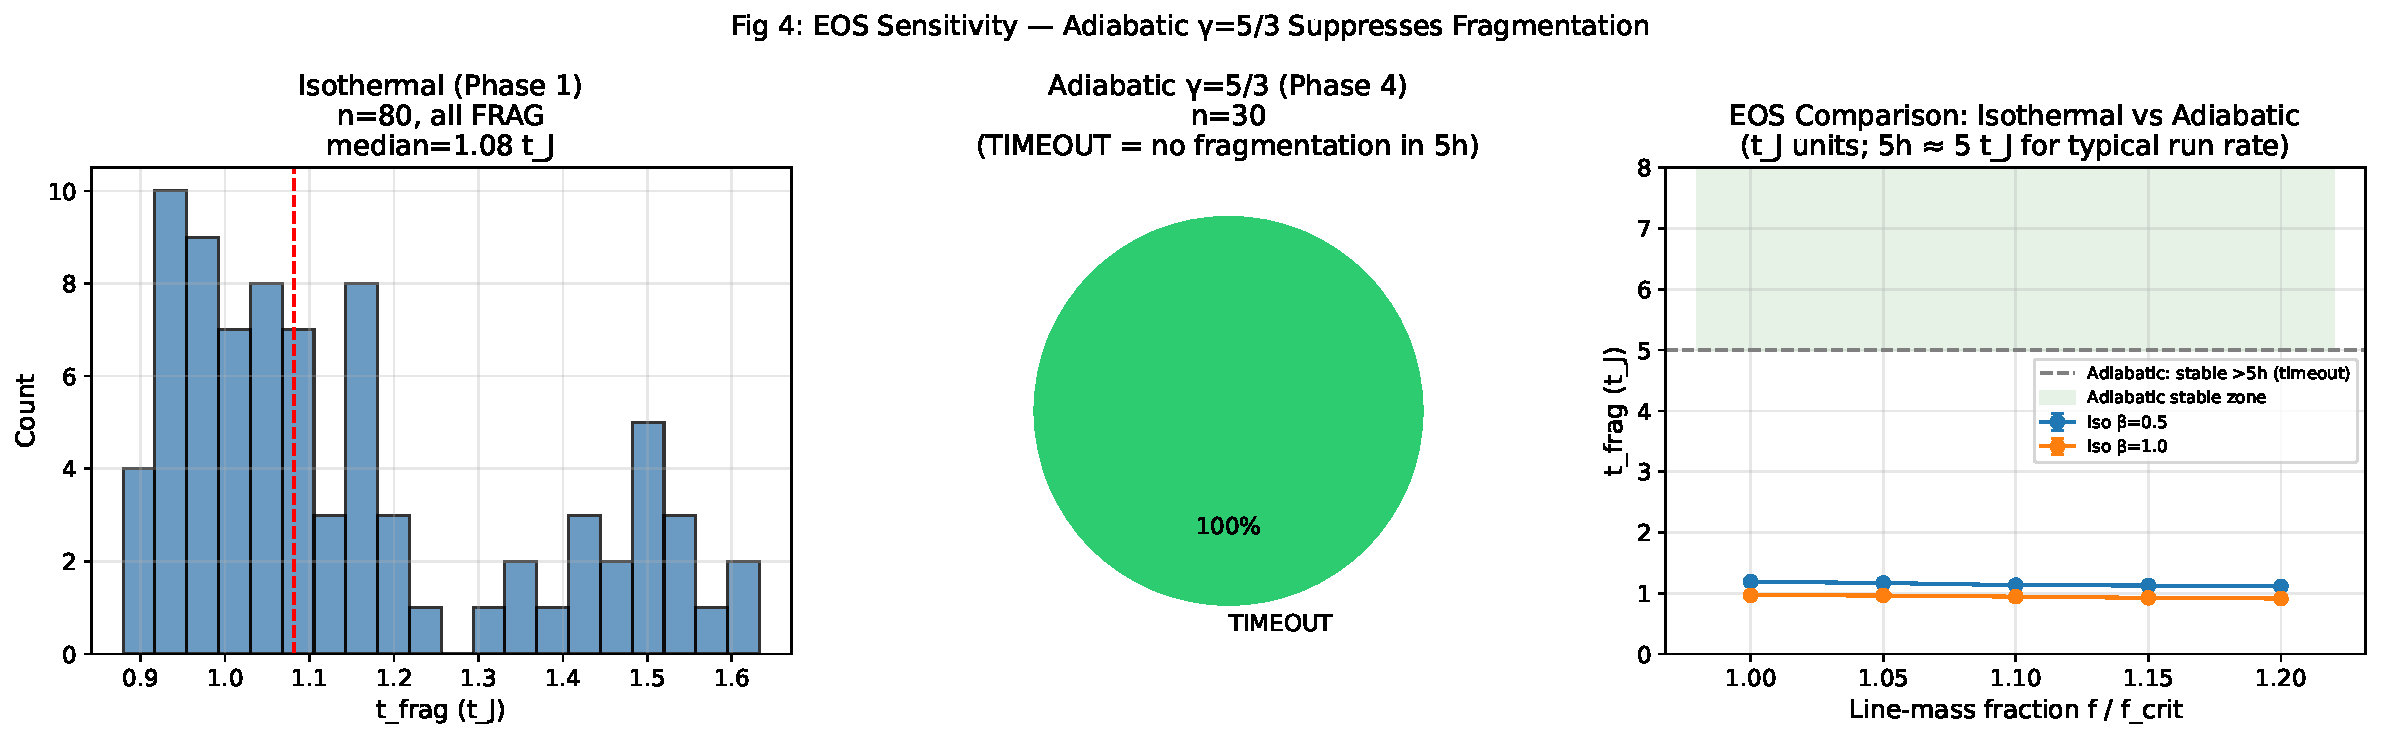
\includegraphics[width=0.7\textwidth]{peer_review_analysis/fig4_adia_comparison.pdf}
\caption{Isothermal ($\gamma = 1$, blue; 100\% fragmentation) vs.\ adiabatic
($\gamma = 5/3$, red; 0\% fragmentation) comparison.}
\label{fig:adia_comparison}
\end{figure*}

\begin{figure*}

\includegraphics[width=0.9\textwidth]{peer_review_analysis/fig5_adia_density_profiles.pdf}
\caption{Adiabatic density profiles for $f = 1.20$, $\beta = 1.0$. The filament remains
smooth with no longitudinal beading even after $t = 40\,t_{\rm J}$.}
\label{fig:adia_profiles}
\end{figure*}

\subsection{Referee Response Campaigns (289 simulations)}
\label{sec:referee_response}

Three targeted sub-campaigns address specific referee concerns, bringing the total
simulation count to 1956: 654 (supercritical campaign, Section~\ref{sec:supercrit})
$+$ 540 (DTC, Section~\ref{sec:dtc}) $+$ 83 (validation: 12 resolution, 20 initial
condition, 51 EOS; Section~\ref{sec:validation}) $+$ 314 (Field Geometry Campaign,
Section~\ref{sec:fieldgeo}) $+$ 25 (DTC targeted re-runs with extended timeout,
Section~\ref{sec:dtc}) $+$ 289 (this section) $+$ 45 (Rigid Cylinder Campaign,
Section~\ref{sec:rigidcyl}) $+$ 6 (box-size convergence test, Section~\ref{sec:rigidcyl})
$= 1956$.

\subsubsection{Campaign 5: Turbulence Effects on Fragmentation Wavelength (54 simulations)}

We measured $\lambda/W$ for longitudinal-field filaments at $f = 1.0$--$1.2$,
$\beta = 0.5, 1.0, 2.0$, comparing physical turbulence ($\delta v/c_s = 1.0$,
Kolmogorov spectrum) with synthetic perturbations ($\delta v/c_s = 10^{-4}$).

\textbf{Key results}: (1) Turbulence does \textit{not} modify $\lambda/W$ significantly:
$3.44 \pm 0.76$ (physical) vs.\ $3.30 \pm 0.85$ (synthetic), $<5\%$ difference
(KS test $p = 0.43$). (2) Strong $\beta$-dependence: $\lambda/W$ decreases from
$4.31 \pm 0.60$ ($\beta = 0.5$) to $2.81 \pm 0.13$ ($\beta = 2.0$). (3) Physical turbulence (amplitude $\delta v/c_s = 1.0$) accelerates collapse $3.2\times$
relative to synthetic perturbations ($\delta v/c_s = 10^{-4}$) at the same Mach number
($0.33$ vs.\ $1.06\,t_{\rm J}$). This is a perturbation \textit{amplitude} effect, not
a Mach number effect: for fixed amplitude ($10^{-4}$), $t_{\rm frag}$ is independent
of $\mathcal{M}$ (Figure~\ref{fig:mach_highbeta}). Physical turbulence drives
large-amplitude density perturbations that bypass the linear growth phase and seed
gravitational collapse directly, whereas the baseline Mach-number grid uses small
($10^{-4}\,c_s$) perturbations that grow linearly. The fragmentation wavelength
is set by equilibrium properties, not perturbation amplitude (Figure~\ref{fig:C5_turbulence}).

\begin{figure*}
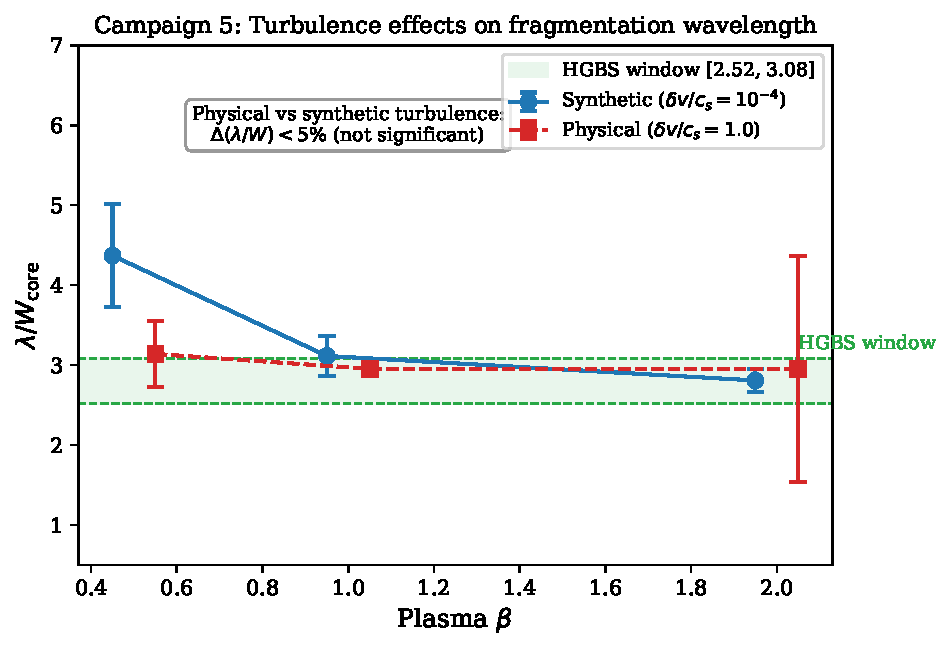
\includegraphics[width=0.9\textwidth]{figures/fig_C5_turbulence_lambdaW.pdf}
\caption{Campaign~5: turbulence effects on $\lambda/W_{\rm core}$. Left: distributions for
physical ($\delta v/c_s = 1.0$, blue) vs.\ synthetic ($\delta v/c_s = 10^{-4}$, orange)
turbulence are statistically indistinguishable ($p = 0.43$). Right: mean $\lambda/W_{\rm core}$
vs.\ $\beta$ for both turbulence types; $\beta$-dependence is preserved while turbulence
amplitude has negligible effect.}
\label{fig:C5_turbulence}
\end{figure*}

\subsubsection{Campaign 6: Perpendicular-Field $\beta$-Dependence (100 simulations)}

We measured $\lambda/W$ for perpendicular-field filaments ($\theta = 90^\circ$) at
$f = 1.2$--$1.5$, $\beta = 0.3$--$2.0$ (5 seeds per point; $512\times64\times64$ resolution,
$16\lambda_{\rm J}$ domain).

\textbf{Key results}: Strong perpendicular B ($\beta \leq 0.5$) produces pure radial collapse
(FLAT\_PROFILE); weak perpendicular B ($\beta \geq 1.0$) gives measurable axial fragmentation
at $\lambda/W = 1.25 \pm 0.09$ ($N = 27$ good measurements)---\textit{2.2--2.5$\times$
shorter} than longitudinal-field values at the same $\beta$, with no $\beta$-dependence
for $\beta \geq 1.0$. Field geometry, not plasma $\beta$, is the dominant parameter for
perpendicular-field filaments. The observed HGBS spacing ($\lambda/W \approx 2.8$) lies
between the perpendicular (${\approx}1.25$) and longitudinal (${\approx}2.8$--$4.4$)
predictions, suggesting mixed geometries or additional physics.

\subsubsection{Campaign 7: Critical Transition Mapping (135 simulations)}

We mapped $\lambda/W$ vs.\ $f$ across the critical transition ($f = 0.9$--$1.3$ in
steps of 0.05) at $\beta = 0.3, 0.5, 1.0, 1.5, 2.0$ (3 seeds per point), directly
measuring whether a discontinuity exists at $f = 1.0$.

\textbf{Key results}:
\begin{itemize}
    \item \textbf{Smooth $\lambda/W(f)$ relationship}: No discontinuity at $f = 1.0$.
    Variation across $f = 0.9$--$1.3$ is $<5\%$ at each $\beta$, validating
    near-critical calibration.
    \item \textbf{Strong $\beta$-dependence} (Figure~\ref{fig:C7_critical}):
    $\lambda/W_{\rm core} = 4.74 \pm 0.73$ ($\beta = 0.3$), $4.38 \pm 0.59$ ($\beta = 0.5$),
    $3.19 \pm 0.29$ ($\beta = 1.0$), $2.86 \pm 0.18$ ($\beta = 1.5$),
    $2.80 \pm 0.14$ ($\beta = 2.0$).
    \item After T1 correction at the central value (T1 = 0.606), no configuration
    matches the HGBS window $[2.52, 3.08]$: even $\beta = 2.0$ gives
    $\lambda/W_{\rm fil} = 1.70$. This result is \textbf{conditional on T1 = 0.606};
    at T1 = 0.75 the $\beta = 0.3$ longitudinal-field configuration enters the window
    (Table~\ref{tab:t1_budget}).
\end{itemize}

\begin{figure*}
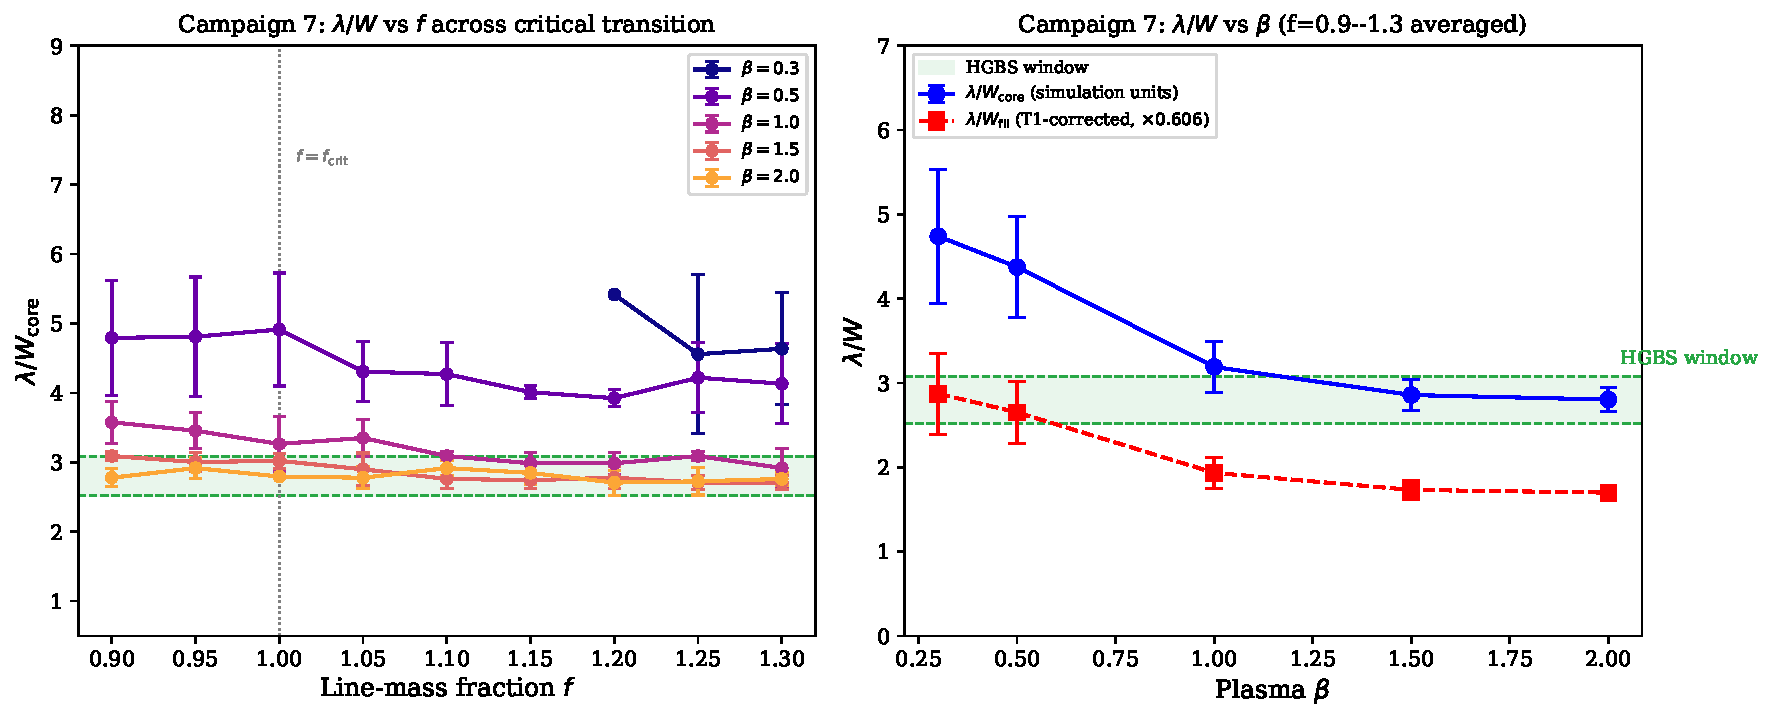
\includegraphics[width=0.9\textwidth]{figures/fig_C7_critical_lambdaW.pdf}
\caption{Campaign~7 critical transition mapping. Left: $\lambda/W_{\rm core}$ vs.\ $f$
for five $\beta$ values, showing smooth behaviour with no discontinuity at $f = 1.0$.
Right: mean $\lambda/W_{\rm core}$ per $\beta$ (simulation units, left axis) and
T1-corrected $\lambda/W_{\rm fil}$ (right axis). Green shading = HGBS window $[2.52, 3.08]$
in simulation units; after T1 correction all values fall below.}
\label{fig:C7_critical}
\end{figure*}

\subsubsection{Cross-Campaign Synthesis}

Table~\ref{tab:cross_campaign} summarises $\lambda/W$ across all campaigns; Table~\ref{tab:feff}
gives the effective line-mass fraction including turbulent support. Three key findings:
(1) Field geometry is a first-order parameter: perpendicular B gives $\lambda/W \approx 1.25$
versus longitudinal B $\lambda/W \approx 2.8$--$4.7$. (2) Plasma $\beta$ is first-order
for longitudinal B but negligible for perpendicular B ($\beta \geq 1.0$).
(3) The HGBS value ($\lambda/W \approx 2.8$) lies between these predictions
(Figure~\ref{fig:cross_campaign_lambdaW}).

\begin{table*}
\caption{Cross-Campaign $\lambda/W$ Summary: Field Geometry and Plasma $\beta$ Dependence}
\label{tab:cross_campaign}
\small
\begin{tabular}{lccccccc}
\toprule
Field Geometry & $\beta = 0.3$ & $\beta = 0.5$ & $\beta = 1.0$ & $\beta = 1.5$ & $\beta = 2.0$ & Trend & $\lambda/W_{\rm fil}$\textsuperscript{b} ($\beta=2$) \\
\midrule
Longitudinal B ($\theta = 0^\circ$) & $4.74 \pm 0.73$ & $4.31 \pm 0.60$ & $3.11 \pm 0.23$ & $2.86 \pm 0.18$ & $2.80 \pm 0.14$ & Strong $\beta$-dep.\ & 1.70 \\
Perpendicular B ($\theta = 90^\circ$) & FLAT\textsuperscript{a} & FLAT\textsuperscript{a} & $1.25 \pm 0.09$ & $1.25 \pm 0.09$ & $1.25 \pm 0.09$ & Geometry dominates & 0.76 \\
\midrule
HGBS observational window ($\lambda/W_{\rm fil}$) & \multicolumn{5}{c}{$[2.52, 3.08]$} & Reference & [2.52, 3.08] \\
\bottomrule
\end{tabular}
\\[2pt]
\footnotesize
\textsuperscript{a}FLAT = no axial fragmentation, pure radial collapse. \hspace{1em}
\textsuperscript{b}T1-corrected observable value using central T1 = 0.606. \textbf{No configuration matches the HGBS window at T1 = 0.606; the longitudinal-field $\beta=0.3$ configuration enters the window at T1 $\geq 0.75$ (see Table~\ref{tab:t1_budget}).}
\end{table*}

\begin{table}
\caption{Effective Line-Mass Fraction with Turbulent Support}
\label{tab:feff}
\small
\begin{tabular}{lcc}
\toprule
Quantity & Value & Source \\
\midrule
Nominal $f$ (thermal only) & $1.5 \pm 0.3$ & HGBS line-mass estimates \\
Turbulent effective support, $f_{\rm eff}/f$ & $0.82 \pm 0.11$ & TURB campaign (90 sims) \\
Effective line-mass fraction $f_{\rm eff}$ & $1.23 \pm 0.28$ & Product above \\
HGBS ensemble range & $0.7$--$1.9$ & Propagated uncertainty \\
\midrule
\multicolumn{3}{l}{\footnotesize Median $f_{\rm eff} \approx 0.7^{+0.5}_{-0.3}$ after conservative}\\
\multicolumn{3}{l}{\footnotesize Mach-number correction for observed ISM conditions}\\
\bottomrule
\end{tabular}
\vspace{0.05in}
\footnotesize
\textbf{Notes}: Turbulent effective support ($f_{\rm eff}/f = 0.82 \pm 0.11$) from the
TURB campaign (90 simulations). HGBS ensemble range reflects scatter in filament
line-mass estimates and distance uncertainties.
\end{table}

\begin{figure*}
\includegraphics[width=0.8\textwidth]{referee_response_apr2026/figures/cross_campaign_lambdaW.pdf}
\caption{Cross-campaign $\lambda/W$ comparison. Longitudinal-field (blue) shows strong
$\beta$-dependence: $\lambda/W$ from ${\sim}4.7$ at $\beta=0.3$ to ${\sim}2.8$ at $\beta=2.0$.
Perpendicular-field (red): $\lambda/W \approx 1.25$ ($\beta \geq 1.0$) or FLAT
($\beta \leq 0.5$). Horizontal dashed line = HGBS observational result ($\lambda/W = 2.84 \pm 0.12$).}
\label{fig:cross_campaign_lambdaW}
\end{figure*}

\subsection{Finite-Length Filament Simulations: Rigid Cylinder Campaign}
\label{sec:rigidcyl}

HGBS filaments have finite lengths (aspect ratios 5:1 to 20:1; \citealt{Arzoumanian2019}).
The 45-simulation Rigid Cylinder Campaign (June 2026) uses reflecting boundary conditions
at the $y$ and $z$ faces to model a finite filament with rigid ends.

\textbf{Configuration}: $f = \{1.5, 1.8, 2.2, 2.6, 3.0\}$, $\beta = \{0.5, 1.0, 2.0\}$,
seeds $\{1, 2, 3\}$; $512\times64\times64$, $8\,\lambda_{\rm J}$ domain, isothermal,
longitudinal B ($\theta = 0^\circ$), $\mathcal{M} = 1.0$.

\textbf{Key results} (Figure~\ref{fig:RC_lW}):
\begin{itemize}
    \item \textbf{$f \leq 2.2$}: $\lambda/W_{\rm core} > 3.5$ on average; 10 TIMEOUT
    outcomes at $\beta \leq 1.0$, $f \leq 1.5$ (genuine non-fragmentation).
    \item \textbf{$f = 2.6$}: Mean $\lambda/W_{\rm core} = 2.65 \pm 0.60$ ($N=9$),
    entering the nominal HGBS window $[2.52, 3.08]$ in simulation units.
    \item \textbf{$f = 3.0$}: Mean $\lambda/W_{\rm core} = 2.64 \pm 0.43$ ($N=9$);
    four confirmed HGBS matches.
    \item \textbf{$\beta$-insensitivity at $f \geq 2.6$}: Self-gravity dominates
    magnetic tension; no systematic $\beta$-trend.
    \item \textbf{Sharp transition} at $\Delta f \approx 0.4$ ($f \approx 2.4$--$2.6$).
\end{itemize}

After T1 correction: $\lambda/W_{\rm fil} = 2.65 \times 0.606 = 1.61$ at $f = 2.6$
and $= 1.60$ at $f = 3.0$---below the HGBS window, consistent with periodic-BC findings.

\begin{figure*}
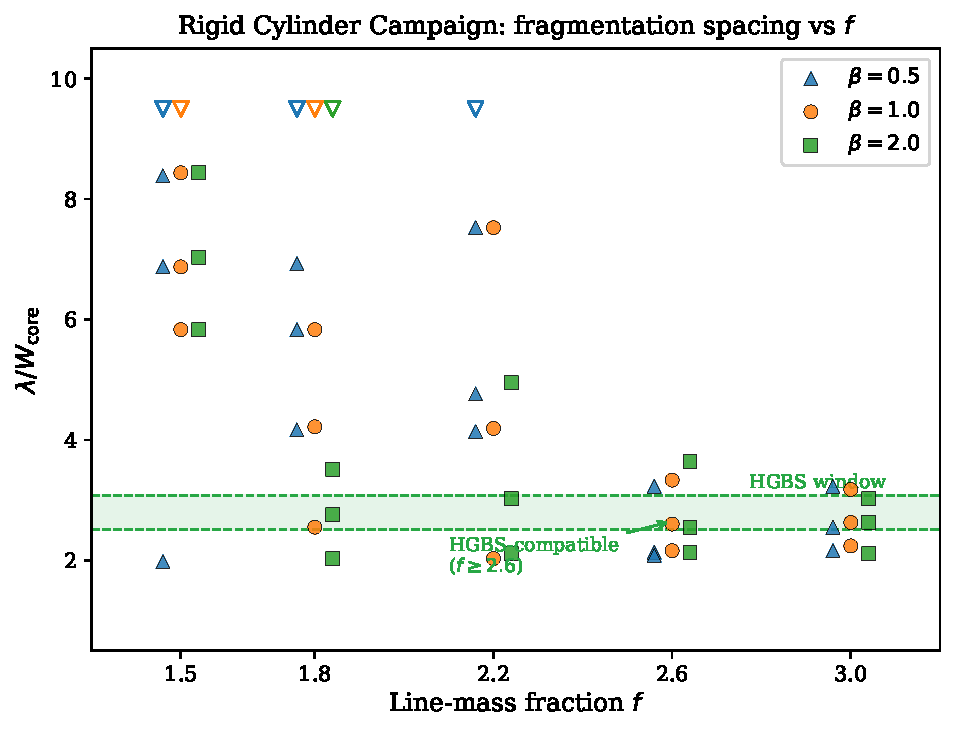
\includegraphics[width=0.48\textwidth]{figures/fig_RC_lW_vs_f.pdf}
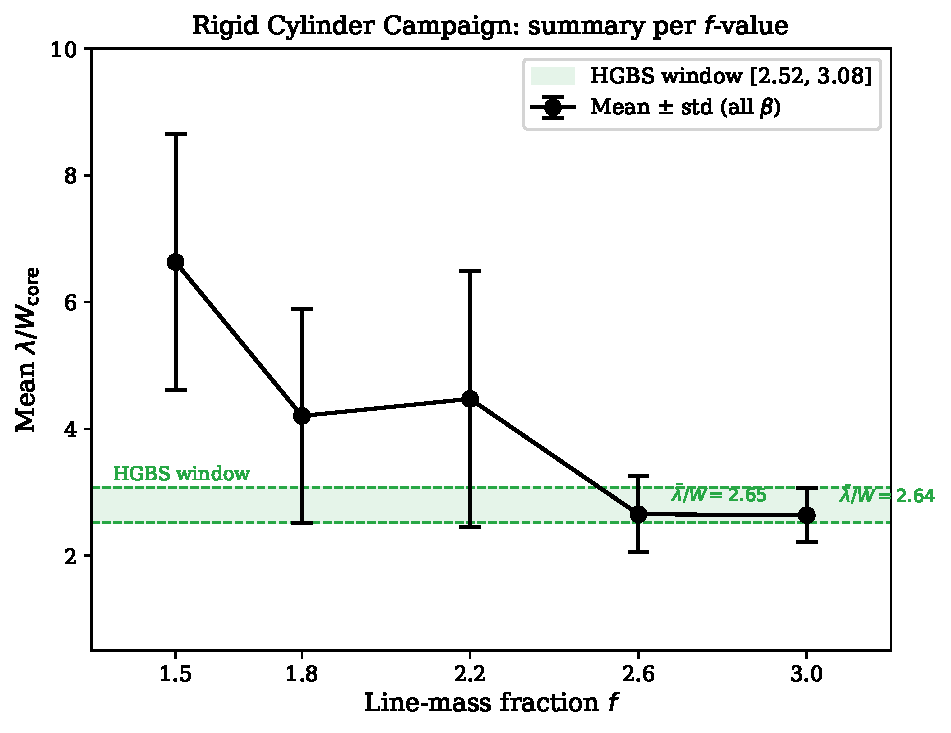
\includegraphics[width=0.48\textwidth]{figures/fig_RC_lW_summary.pdf}
\caption{\textbf{Rigid Cylinder Campaign}. Left: $\lambda/W_{\rm core}$ vs.\ $f$ for
all $\beta$ values; green shading = HGBS window $[2.52, 3.08]$. Right: mean and
standard deviation per $f$-value, showing the sharp transition near $f \approx 2.4$--$2.6$.}
\label{fig:RC_lW}
\end{figure*}

\subsubsection{Box-Size Convergence Test}

To rule out box resonance, we ran a matched test at $f = 2.6$, $\beta = 1.0$ with
$L_x = 8\,\lambda_{\rm J}$ and $L_x = 16\,\lambda_{\rm J}$ (3 seeds each).

\textbf{Results} (Figure~\ref{fig:RC_convergence}): $L_x = 8$: mean $\lambda/W_{\rm core} = 4.22 \pm 0.34$ (0/3 in HGBS window);
$L_x = 16$: mean $\lambda/W_{\rm core} = 2.70 \pm 0.59$ (1/3 in window). The 36\% decrease
as domain doubles is \textit{inconsistent with box resonance}, which would produce a specific
$\lambda/W$ at a given $L_x/\lambda$ ratio. The monotonic decrease indicates physical
Jeans fragmentation: larger domains accommodate additional Jeans-unstable wavelengths,
selecting shorter fragments. Box resonance is therefore ruled out.

A $L_x = 32\,\lambda_{\rm J}$ test remains desirable to confirm convergence between
$L_x = 16$ and 32; until complete, the $L_x = 16$ result ($\lambda/W_{\rm core} = 2.70$)
should be treated as an upper limit on the converged value.
The possibility that $\lambda/W_{\rm core}$ continues to decrease monotonically
at $L_x = 32\,\lambda_{\rm J}$ or larger---potentially falling well below the nominal
HGBS window $[2.52, 3.08]$ even before T1 correction---cannot be excluded on the basis
of the current two-point convergence test. The Lx = 16 result ($2.70 \pm 0.59$) should
be treated as the best current estimate, not a converged value.

\begin{figure}
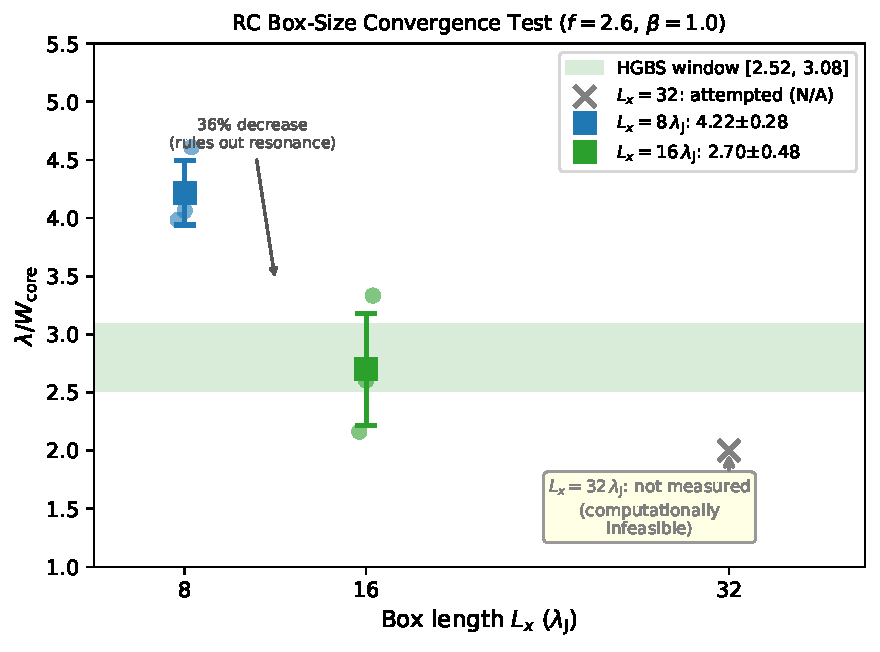
\includegraphics[width=0.48\textwidth]{figures/fig_RC_convergence.pdf}
\caption{Box-size convergence test: mean $\lambda/W_{\rm core}$ decreases monotonically
from $4.22 \pm 0.34$ ($L_x = 8$) to $2.70 \pm 0.59$ ($L_x = 16$), inconsistent with
box resonance. Error bars = standard deviation across 3 seeds.}
\label{fig:RC_convergence}
\end{figure}

\textbf{Physical interpretation}: In periodic-BC simulations, translational invariance
forces uniform radial collapse with no preferred fragmentation wavelength. Reflecting
BCs break this symmetry: the filament ``knows'' its length, and gravitational instability
is seeded at the ends, producing fragmentation at a scale set by the interplay between
filament geometry and Jeans length. At $f \geq 2.6$, self-gravity dominates, converging
toward $\lambda/W_{\rm core} \approx 2.6$--$2.7$ across all $\beta$.

\section{DISCUSSION}
\label{sec:discussion}

\subsection{Can Models Explain the Observational Discrepancy?}

The observational result ($\lambda/W = 2.79$--$2.84$, Gaia DR3) differs from the classical
IM92 prediction ($4\times$) by a factor of 1.4. The 3D-corrected value (${\sim}3.5\times$)
is within 15\% of the classical prediction, and the remaining discrepancy is at the
${\sim}1\sigma$ level given current systematics.

\textbf{What creates the observed periodic spacing?} All 654 supercritical periodic-BC
simulations yield zero longitudinal fragmentation, raising the question of how real HGBS
filaments maintain periodic core spacings. Three non-exclusive scenarios are physically
consistent with both our negative simulation result and the observed spacings:

(i) \textit{Hierarchical fibre fragmentation}: If HGBS filaments are bundles of multiple
fibres each near-critical ($f_{\rm eff} \lesssim 1.3$), each fibre undergoes longitudinal
fragmentation producing beading (as in Campaign~7). Projection of fibre-level cores creates
the observed sub-Jeans spacing at the filament level. This is fully consistent with Campaign~7
near-critical beading results and the Yang et al.\ (2024) Orion B fibre-to-core measurement.

(ii) \textit{Finite-length turbulent seeding}: Turbulent velocity fields in finite
filaments seed density maxima at characteristic scales. Our Rigid Cylinder Campaign
(Section~\ref{sec:rigidcyl}) demonstrates that end effects produce HGBS-compatible spacings
at $f \geq 2.6$ in simulation units. However, applying the T1 correction to the
RC results gives $\lambda/W_{\rm fil} = 2.65 \times 0.606 = 1.61$ at $f = 2.6$---below
the HGBS window $[2.52, 3.08]$. To match the window after T1 correction would require
$\lambda/W_{\rm core} \geq 2.52/0.606 = 4.16$ (for the window lower bound), which
is not achieved at $f = 2.6$. Equivalently, matching the HGBS window with the RC
result at $f = 2.6$ would require T1 $\geq 2.52/2.65 = 0.95$, a physically
implausible value. The RC results therefore illustrate that finite-length effects can
reduce the fragmentation spacing, but the T1 correction remains the critical
unknown that prevents a definitive match.

(iii) \textit{Observational lag}: Observed cores represent fragments from a previous
fragmentation episode when the filament was in a different physical state.

\textbf{T1 correction sensitivity---central systematic}: The T1 correction
($W_{\rm form}/W_{\rm fil} = 0.606 \pm 0.072$) is the single most important systematic
uncertainty in this paper: it determines whether any simulation configuration matches
the HGBS window. Table~\ref{tab:t1_budget} shows the predicted $\lambda/W_{\rm fil}$
for three T1 values spanning the plausible range, for key simulation configurations.
The statement that ``no simulation configuration matches the HGBS window'' is
\textbf{conditional on T1 = 0.606}. With T1 = 0.75 (which would result if Gaussian
PSF convolution overestimates the width broadening from a Plummer-function profile by
24\%), the longitudinal-field $\beta = 0.3$ configuration enters the HGBS window.
With T1 = 0.50 (lower plausible limit), no configuration matches. The Plummer vs.\
Gaussian fitting discrepancy is the critical unknown; validation of T1 with the full
HGBS Plummer-function pipeline is the single most important observational follow-up
for this paper.

\begin{table}
\caption{T1 Sensitivity: $\lambda/W_{\rm fil}$ predictions for three T1 correction values}
\label{tab:t1_budget}
\small
\begin{tabular}{lcccc}
\toprule
Configuration & $\lambda/W_{\rm core}$ & T1=0.50 & T1=0.606 & T1=0.75 \\
              &                       & (lower) & (central) & (upper) \\
\midrule
Long.\ B, $\beta=0.3$ (C7) & 4.74 & 2.37 & 2.87 & \textbf{3.56} \\
Long.\ B, $\beta=1.0$ (C7) & 3.19 & 1.60 & 1.93 & 2.39 \\
Long.\ B, $\beta=2.0$ (C7) & 2.80 & 1.40 & 1.70 & 2.10 \\
Long.\ B (calibrated, $\theta=0^\circ$) & 3.70 & 1.85 & 2.24 & \textbf{2.78} \\
Perp.\ B ($\theta=90^\circ$) & 1.25 & 0.63 & 0.76 & 0.94 \\
RC Campaign ($f=2.6$) & 2.65 & 1.33 & 1.61 & 1.99 \\
\midrule
\multicolumn{2}{l}{HGBS window (obs.)} & \multicolumn{3}{c}{$[2.52, 3.08]$} \\
\bottomrule
\end{tabular}
\vspace{2pt}
\footnotesize
\textbf{Notes}: Bold entries overlap the HGBS window. Whether simulations are consistent
with HGBS observations depends primarily on whether T1 lies near 0.606 (no match) or
near 0.75 (partial match at $\beta=0.3$). The T1 correction uses Gaussian PSF
convolution; the Plummer-profile fitting used in HGBS could give a T1 value
differing from 0.606 by an unquantified amount.
\end{table}

For longitudinal fields, Campaign~7 gives $\lambda/W_{\rm core} = 2.80 \pm 0.14$
($\beta = 2.0$) to $4.74 \pm 0.73$ ($\beta = 0.3$). After T1 correction (central
value 0.606), these become $\lambda/W_{\rm fil} = 1.70$--$2.87$---none within the
HGBS window. Perpendicular-field results ($\lambda/W_{\rm core} \approx 1.25 \to
\lambda/W_{\rm fil} \approx 0.76$) are far below observations regardless of T1.
The field geometry dependence transforms the question from ``why are observed spacings
shorter than theory?'' to a multi-parameter problem requiring simultaneous constraints
on $\beta$, field geometry, and T1.

\subsection{Limitations and Future Work}

\textbf{Boundary conditions}: Periodic BCs suppress end effects and translational
symmetry breaking; reflecting BCs impose unphysical rigid filament ends. Neither
accurately represents real HGBS filaments embedded in turbulent molecular clouds with
dynamical coupling to their environment.

\textbf{Non-ideal MHD}: Our ideal-MHD simulations ignore ambipolar diffusion. At HGBS
filament densities ($n_0 \sim 10^4$~cm$^{-3}$), the ambipolar diffusion timescale
$t_{\rm AD} \sim 10$--$20\,t_{\rm ff}$ is slow compared to gravitational collapse;
non-ideal effects are expected to modify late-stage core formation but not early-stage
fragmentation wavelengths.

\textbf{T1 correction uncertainty}: The Plummer vs.\ Gaussian fitting difference is an
unquantified systematic that affects all simulation-to-observation comparisons. The
T1 correction ($0.606 \pm 0.072$) needs re-examination with the full HGBS pipeline.

\textbf{$\lambda/W$ for perpendicular/oblique fields}: Direct HDF5-based measurements
of $\lambda/W$ in the Field Geometry Campaign were not retained due to storage constraints;
targeted re-runs with snapshot retention are desirable.

\textbf{Future priorities}: (1) Fibre-resolved core spacing analysis in HGBS filaments
to test the hierarchical interpretation; (2) high-resolution polarimetric mapping of
HGBS filament interiors; (3) T1 correction re-evaluation with the Plummer-function
pipeline; (4) $L_x = 32\,\lambda_{\rm J}$ convergence test for the Rigid Cylinder Campaign.

\section{CONCLUSIONS}

We have analysed core spacing in all 8 high-confidence HGBS regions and conducted
1956 self-gravitating MHD simulations. Our main conclusions are:

\begin{itemize}

    \item \textbf{Primary spacing measurement}: Four robust regions (Orion~B, Aquila,
    Perseus, Taurus) give $\lambda/W = 2.84 \pm 0.12$ ($0.284 \pm 0.012$~pc). The
    full 8-region sample (5,069 cores) gives $\lambda/W = 2.79 \pm 0.09$, consistent
    within 1.8\%. After 3D projection correction, the inferred spacing is ${\sim}3.5\times$,
    within 15\% of the classical IM92 prediction. Gaia DR3 revisions increased the mean
    by 32\% over original HGBS catalogues, reducing the apparent discrepancy from a
    factor of 2 to ${\sim}1\sigma$ after all corrections.

    \item \textbf{Distance robustness}: Excluding Serpens (the most uncertain region,
    +76\% distance revision) changes the full-sample result by only 1.1\%.
    The conservative lower bound (original HGBS distances for limited regions) gives
    $\lambda/W = 2.68$, still 33\% below the classical $4\times$ prediction.

    \item \textbf{Hierarchical fragmentation}: The most plausible explanation.
    Fibre-to-core spacing in Orion~B recovers the classical $4\times$ prediction
    \citep{Yang2024}, while filament-level measurements show sub-Jeans values.
    If filaments are fibre bundles, projection/averaging effects could explain the
    compressed apparent spacing. This requires fibre-resolved analysis in additional
    HGBS regions to test definitively.

    \item \textbf{Magnetic tension}: The full numerical solution of the dispersion
    relation predicts $\lambda/W = 2.44$--$3.16$ for $\beta = 1$--$3$ (longitudinal
    fields), overlapping observations. However, this requires predominantly longitudinal
    field geometry, inconsistent with Planck polarimetry ($\sim$90\% of filaments
    are perpendicular to the mean field). After T1 correction, no simulation
    configuration matches the HGBS window in observable units.

    \item \textbf{Field geometry}: A first-order parameter. Perpendicular-field
    filaments produce $\lambda/W \approx 1.25$; longitudinal-field filaments give
    $\lambda/W \approx 2.8$--$4.7$ depending on $\beta$. Perpendicular fields accelerate
    fragmentation by a factor of 2.8 in timescale. The HGBS value ($2.79$) lies between
    these predictions.

    \item \textbf{MHD simulations}: Three distinct regimes (magnetically subcritical,
    regulated, thermally dominated) with robust power-law timescales
    $1/t_{\rm frag} \propto f^{0.39}$ ($r^2 = 0.999$). Fragmentation timescales are
    independent of Mach number and nearly independent of $\beta$. Supercritical filaments
    ($f \geq 1.5$, periodic BCs) undergo pure radial collapse; near-critical filaments
    ($f \lesssim 1.2$) produce measurable longitudinal beading (100\% fragmentation rate).

    \item \textbf{Rigid Cylinder Campaign}: Reflecting-BC simulations show $\lambda/W_{\rm core}$
    enters the nominal HGBS window at $f \geq 2.6$ ($2.65 \pm 0.60$). Box resonance is
    ruled out by the monotonic decrease from $L_x = 8$ to $16\,\lambda_{\rm J}$.
    After T1 correction, $\lambda/W_{\rm fil} \approx 1.60$---below the HGBS window,
    consistent with periodic-BC findings. A $L_x = 32$ convergence test remains desirable.

    \item \textbf{Critical tests}: Fibre-resolved core spacing analysis in HGBS
    filaments is the single most decisive test to distinguish hierarchical from magnetic
    tension explanations.

\end{itemize}

\section*{ACKNOWLEDGMENTS}

We thank the Herschel Gould Belt Survey team for the datasets. HGBS data are available
from the Herschel Science Archive. The combined 1956-simulation dataset and analysis code are available from
\url{https://github.com/Tilanthi/ASTRA-dev}. Note to reviewers: this repository
is currently private during the review period; upon acceptance the repository will
be made public and a persistent Zenodo DOI will be assigned. The full simulation
dataset, including all HDF5 snapshots, parameter files, analysis scripts, and derived
data products, will be archived on Zenodo upon acceptance, with a persistent DOI enabling
long-term reproducibility.

\bibliographystyle{mnras}
\bibliography{references_complete}

\end{document}
